\chapter{Analysis of an interesting \acrshort{ame} region: $\lambda$~Orionis}
\label{ch:lori}
  This chapter is an analysis of the \acrshort{ame} and how it relates to the dust emisison, in the $\lambda$~Orionis region. This has been an ongoing collaboration with F. Galliano, an expert in dust \acrshort{sed} fitting and developer of a dust \acrshort{sed} framework presented in \cite{galliano18}. This work has been enabled by mutual collaboration vists by myself and F. Galliano, funded in part by a joint JSPS-CNRS international collaboration grant. The results described here are intended to form the core of a journal publication, to be submitted in the coming months.

 \section{An interesting \acrshort{ame} region}
		The $\lambda$~Orionis molecular ring, also known as the Meissa Ring is a massive stucture surrounding the $\lambda$~Orionis O-type star. The ring contains an HII region, ionized by $\lambda$Ori itself and its OB associates \citep{murdin77}. What had been thought of as a star\-forming region of missing molecular gas. At the time \cite{murdin77} even speculated that this could be evidence of an alternate star\-formation pathway, writing: ``Notably we need to know if $\lambda$Ori is an example of a different mode of star formation or [...] simply a case in which the progenitor molecular cloud was exhausted within the last one or two million years.''

    \cite{maddalena86,maddalena87}.  (and references therein) noted a ring of material likely being pushed out by the central, historically well-known $\lambda$~Orionis Association of B-type stars and surrounding HII reigon.


    \cite{cunha96} argued that the ring shape around $\lambda$~Orionis may have resulted from a supernova explosion, further speculating that $\lambda$Ori may have been a companion of the progenitor. $\lambda$~Orionis is a known binary system, however its current companion is a B-type star. \citep{murdin77}
  .
     The central region is heated by the $\lambda$~Orionis star itself, and the Orion~OB association it belongs to \citep{ochsendorf15}. The region is known to host several young stellar and protostellar objects \citep{koenig15}.

    At approx. 10$^{\circ}$ wide, we can see the outline of the structure even in the low (1$^{\circ}$ FWHM) resolution PCAME map. The ring shape itself is thought to originate from a supernova, or perhaps combined effects of the entire star formation history of the $\lambda$~Orionis Association, including the formation of its surrounding HII region \citep{aran09}.

    Although the $\lambda$~Orionis region has been a popular target for study since approximately the 1980s. \cite{duerr82} wrote of the relative lack of work on the overall region: ``Surprisingly, this interesting complex has been little studied''. While this seems surprising given the numbe of works on the region in the literature now, it is really the advent of all-sky missions that have driven more recent interest.  The large angular size is such that all-sky surveys were a natural boon for study of such extended structures. WISE especially was a huge source of insight \citep{koenig15}. More recently, \cite{planck15XXV} strongly highlighted the region as a strong candidate for further \acrshort{ame} investigation.

\section{Investigative approach}
  We have carried out an initial comparison of the \acrshort{ame} of this region with its mid to far-IR dust emission. The region is shown in Fig.~\ref{fig:orionis-akari9} as it appears in 1$^{\circ}$-smoothed A9 data.
      \begin{figure}
        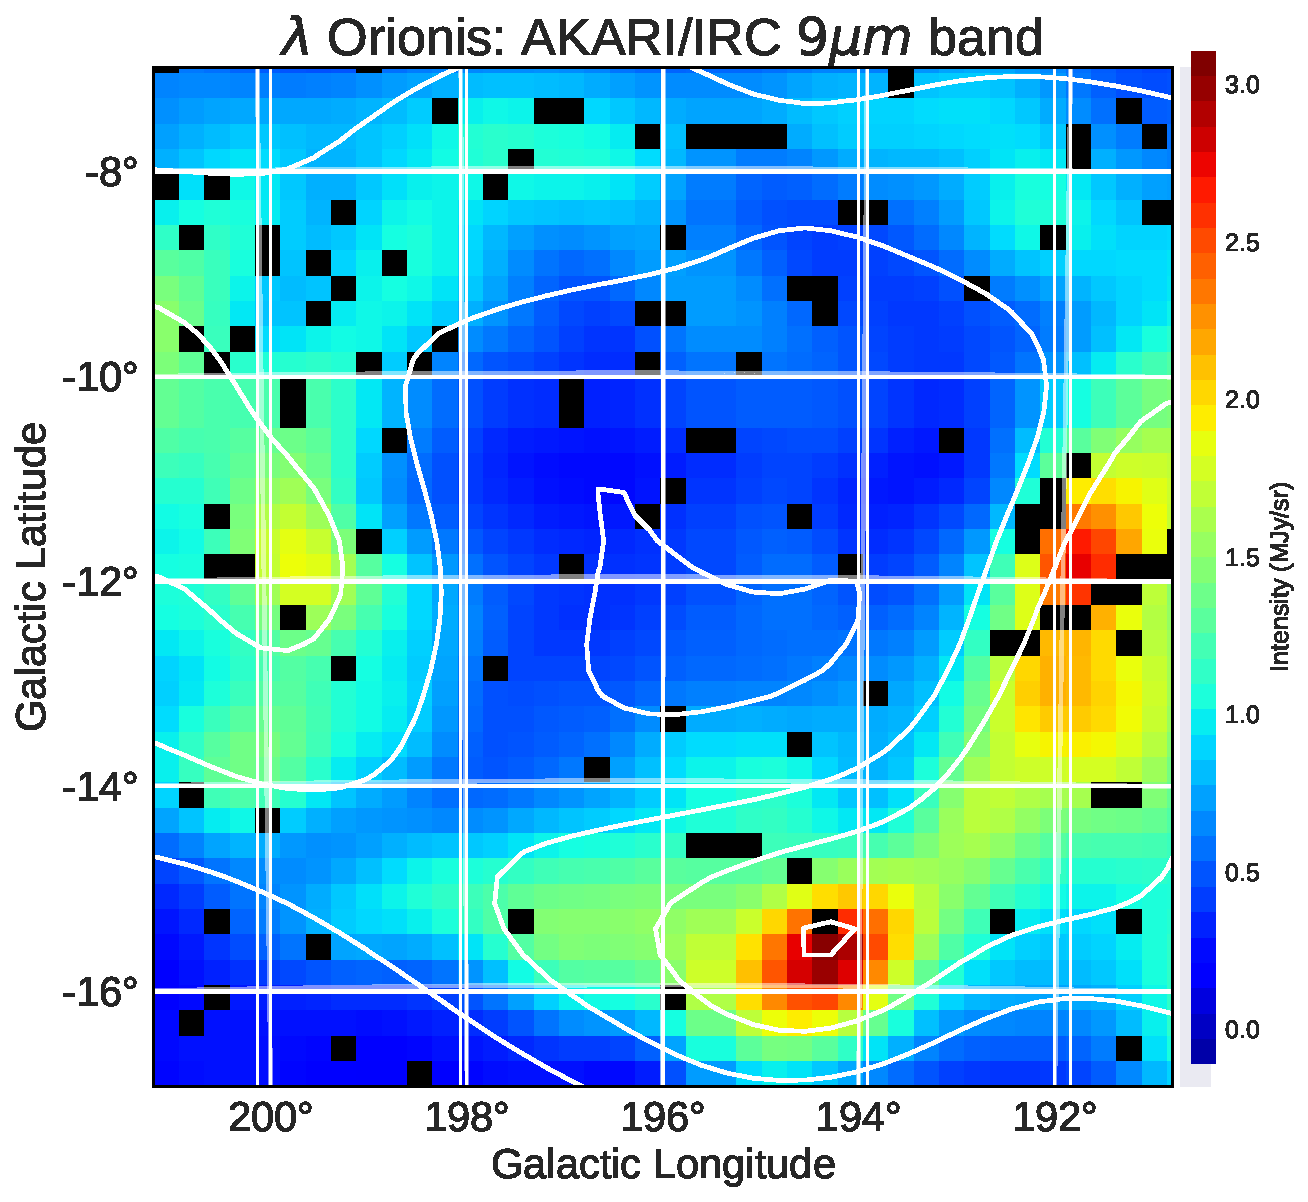
\includegraphics[width=\textwidth]{../Plots/LOri_akari9_AMEcont_1dres.pdf}
        \centering
        \caption{$\lambda$~Orionis as it appears in the AKARI 9~$\mu$m data. Contours indicate the \acrshort{ame}, as given by the Planck PR2 \acrshort{ame} map. The image is smoothed to a 1$^{\circ}$ PSF (much larger than the original 10 arcsec map). The $\lambda$~Orionis star itself is approximately located at the center of the image.}
        \label{fig:orionis-akari9}
      \end{figure}
   The ring structure itself indicates excess microwave emission attributed to \acrshort{ame}, from the dominant variable frequency component $AME_{var}$ (see Ch.~\ref{ch:datasources}). The central region is dominated by free-free emission \citep{aran09, koenig15}. Free-free emisison coming from the Hii phase surrounding the $\lambda$~Orionis association dominates the region's morphology in \acrshort{lfi} images. \citep{planck15XXV}. Taking the hint from \cite{planck15XXV} that this may be among the more reliably component separated regions, we evaluate if there is any preferential relationship between any parameter of dust emission and the \acrshort{ame}. Fig.~\ref{fig:LOri_halpha_AMEvarContours} shows the expected distribution of free-free emission in the region, assuming that $H\alpha$ line emission is a tracer of microwave free-free. This indicates that free-free is strong within the central region, where radiation fields are more intense, and \acrshort{ame} is minimal. The strongest \acrshort{ame} follows the ring-shaped morphology outside the central bubble of free-free emission.
     \begin{figure}
       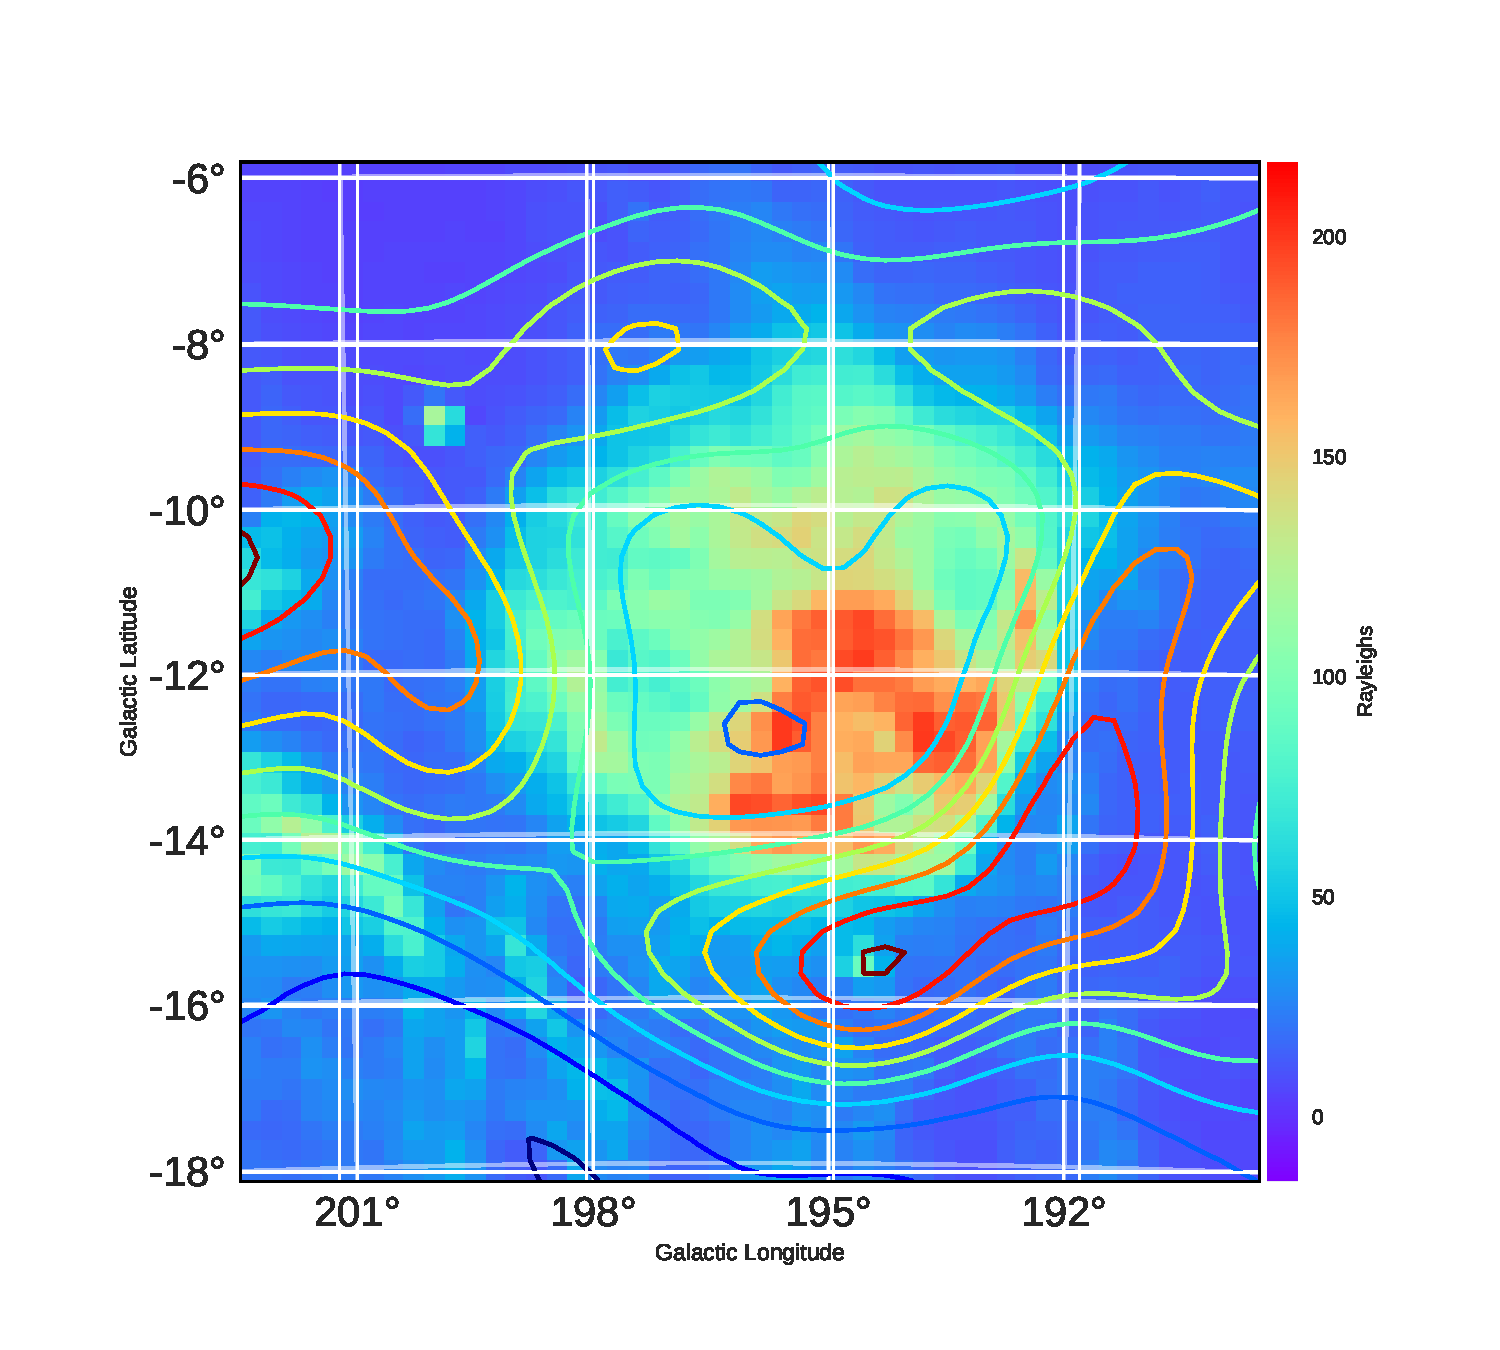
\includegraphics[width=\textwidth]{../Plots/ch_lori/LOri_halpha_AMEvarContours.pdf}
       \centering
       \caption{$\lambda$~Orionis as it appears in H-alpha emission by \cite{finkbeiner03}. Contours indicate \acrshort{ame} emission, from the variable frequency component. The colorbar indicates $H\alpha$ emission in Rayleighs. The field of view is slightly larger than that used for the final processed IR comparison (Fig.~\ref{fig:lori_processed_all}). }
       \label{fig:LOri_halpha_AMEvarContours}
     \end{figure}
    We will first show a model-independent analysis, comparing IR photometric intensities from the mid to far-IR to the \acrshort{ame}. After comparing all of these intensities, we describe which wavelength shows the best intensity correlation. The core results however will be based on a dust SED model-dependent analysis, which takes into consideration all of the photometric intensities to fit the total abundance of dust, PAH abundance, PAH ionization fraction, and ISRF strength, $U$, accross the $\lambda$~Orionis region. We will then discuss the core result, suggesting that PAH mass has a stronger relationship with AME than the total dust mass does, representing the first time such a result has been found for a specific \acrshort{ame}-prominent region.

	\section{Data preparation}
    \label{sec:dataprocessing}
		As indicated in Ch.~\ref{ch:datasources}, we use 12 photometric all-sky maps. For the IRC data (A9 and A18), we produce mosiacs of $\lambda$~Orionis from the latest version of the individual tiles provided internal all-sky archive. A9 and A18 images are produced by regridding the images with the {\tt Montage} software by \acrshort{nasa}/\acrshort{ipac}. Figs.~\ref{fig:lori_A9_mosaic_smooth} and~\ref{fig:lori_A18_mosaic_smooth} show high resolution mosaics of the A9 and A18 data before processing.
      \footnote{IRC all-sky data is still in the proprietary phase at the time of this writing, but should be public by April 2018.}
       For the other sources, HEALPix all-sky maps are available publicly, at sufficient resolution relative to their native resolutions\footnote{Planck data was retreived from the NASA IPAC online archive at \url{http://irsa.ipac.caltech.edu/data/Planck/release_2/all-sky-maps/}}. \footnote{AKARI/FIS data }\footnote{IRAS/IRIS data }

		  Other data were obtained from publically archived HEALPix maps. This includes data from \acrshort{iras}, Planck, \acrshort{dirbe}, and AKARI/FIS. For For these data, we employ the {\tt healpix2wcs} functionality provided in the {\tt gnomdrizz} python package\footnote{Available at \url{http://cade.irap.omp.eu/dokuwiki/doku.php?id=software}}\footnote{``drizzlib'' 1.2.2 and earlier were not able to correctly access HEALPix files with multiple fields/columns. See appendix for our recommended workaround.}   When the extraction and regridding are finished, all of the images --- those extracted from \acrshort{healpix} maps, as well as the \acrshort{irc} data --- share a common FITS header having a pixel grid spacing equal to the average pixel width in the NSIDE 256 \acrshort{healpix} scheme, or about \textasciitilde{0.25$^{\circ{}}$}. After PSF smoothing, described in detail below, the data also have a common \textasciitilde{1$^{\circ{}}$} FWHM effective PSF. Although this means that the grid is oversampled, we choose this approach to preserve as much of the structure of the region as possible, even after masking bad pixels. Another option would be to interpolate the bad pixels, and degrade the pixel scale to the PSF size. However we choose the former method due to the relative large number of bad pixels, especially around the regions affected by missing stripes. This means that in the analyses that follow, what is important is the relative trends between correlation coefficients, rather than their absolute values.

      \subsection{Point-source and artifact masking}

        \paragraph{Missing stripes}
          The AKARI all-sky survey suffers from a few missing stripe errors throughout the \acrshort{irc} and \acrshort{fis} maps \citep{ishihara10, doi15}. This is a more serious issue for \acrshort{fis}. Unfortunately for the present work, some of these stripes pass directly through the $\lambda$~Orionis region. Figs.~\ref{fig:LOri_FIS_color},~\ref{fig:lori_A9_mosaic_smooth} and ~\ref{fig:lori_A18_mosaic_smooth} display the data at near-native resolution, demonstrating where these patterns occur. Additionally there are some saturated pixels in both \acrshort{irc} and \acrshort{fis} data.
            \begin{figure}
              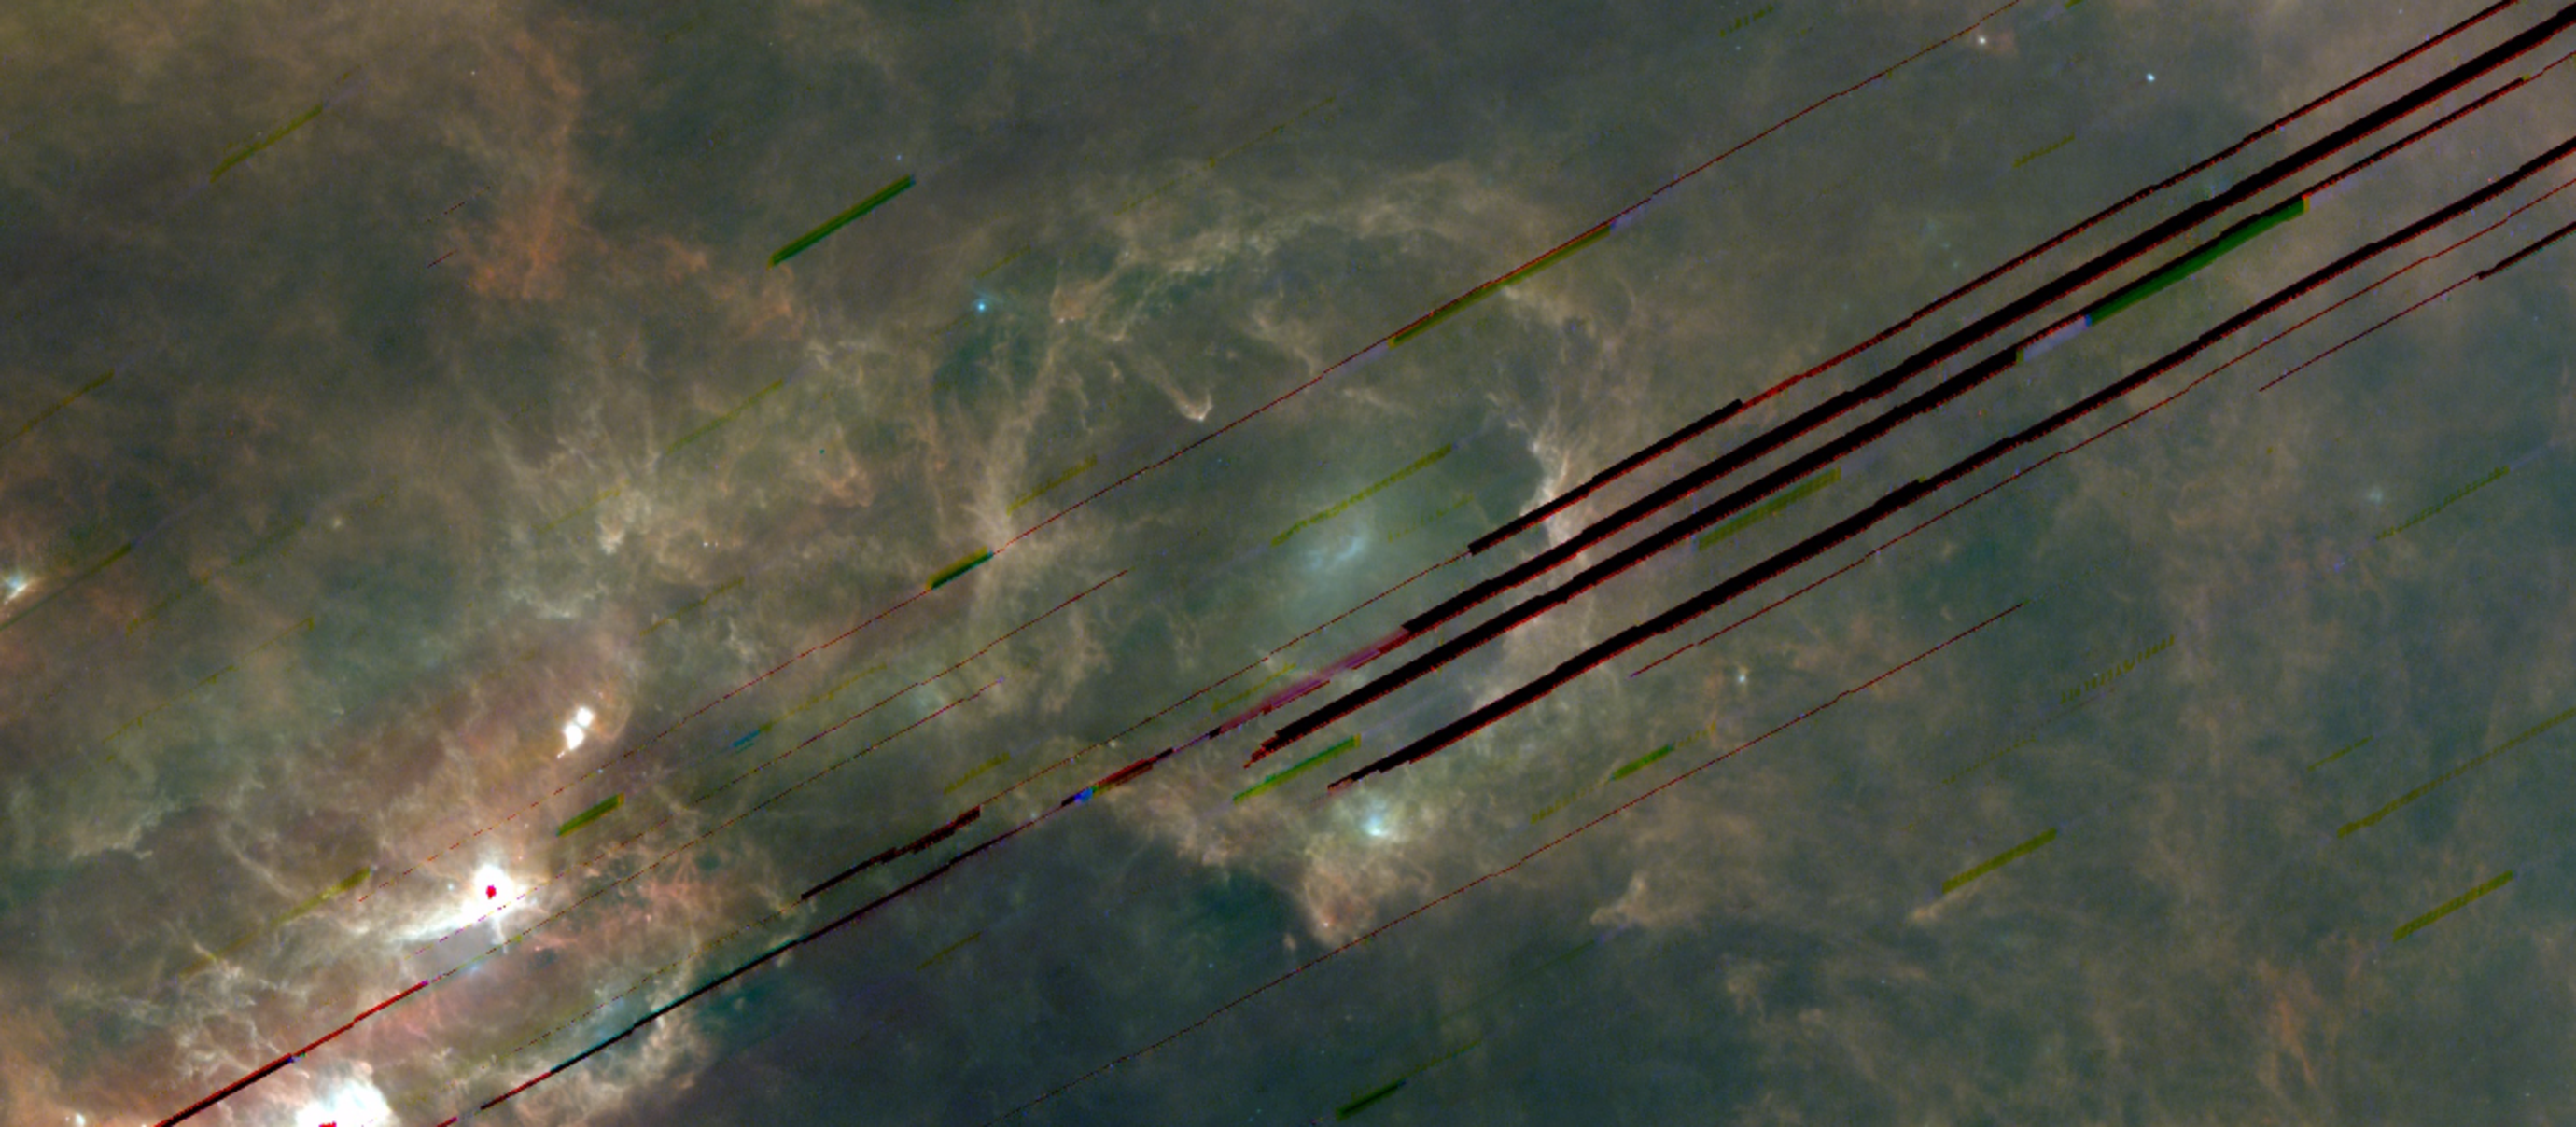
\includegraphics[width=\textwidth]{../Plots/ch_lori/lori_fis_rgb.pdf}
              \centering
              \caption{The $\lambda$~Orionis region and its surroundings in AKARI \acrshort{fis} data, where A65 is blue, A90 is green, and A140 is red. The missing stripe patterns are visible, and affect all 3 bands shown here as well as the A160 data. }
              \label{fig:LOri_FIS_color}
            \end{figure}
            \begin{figure}
              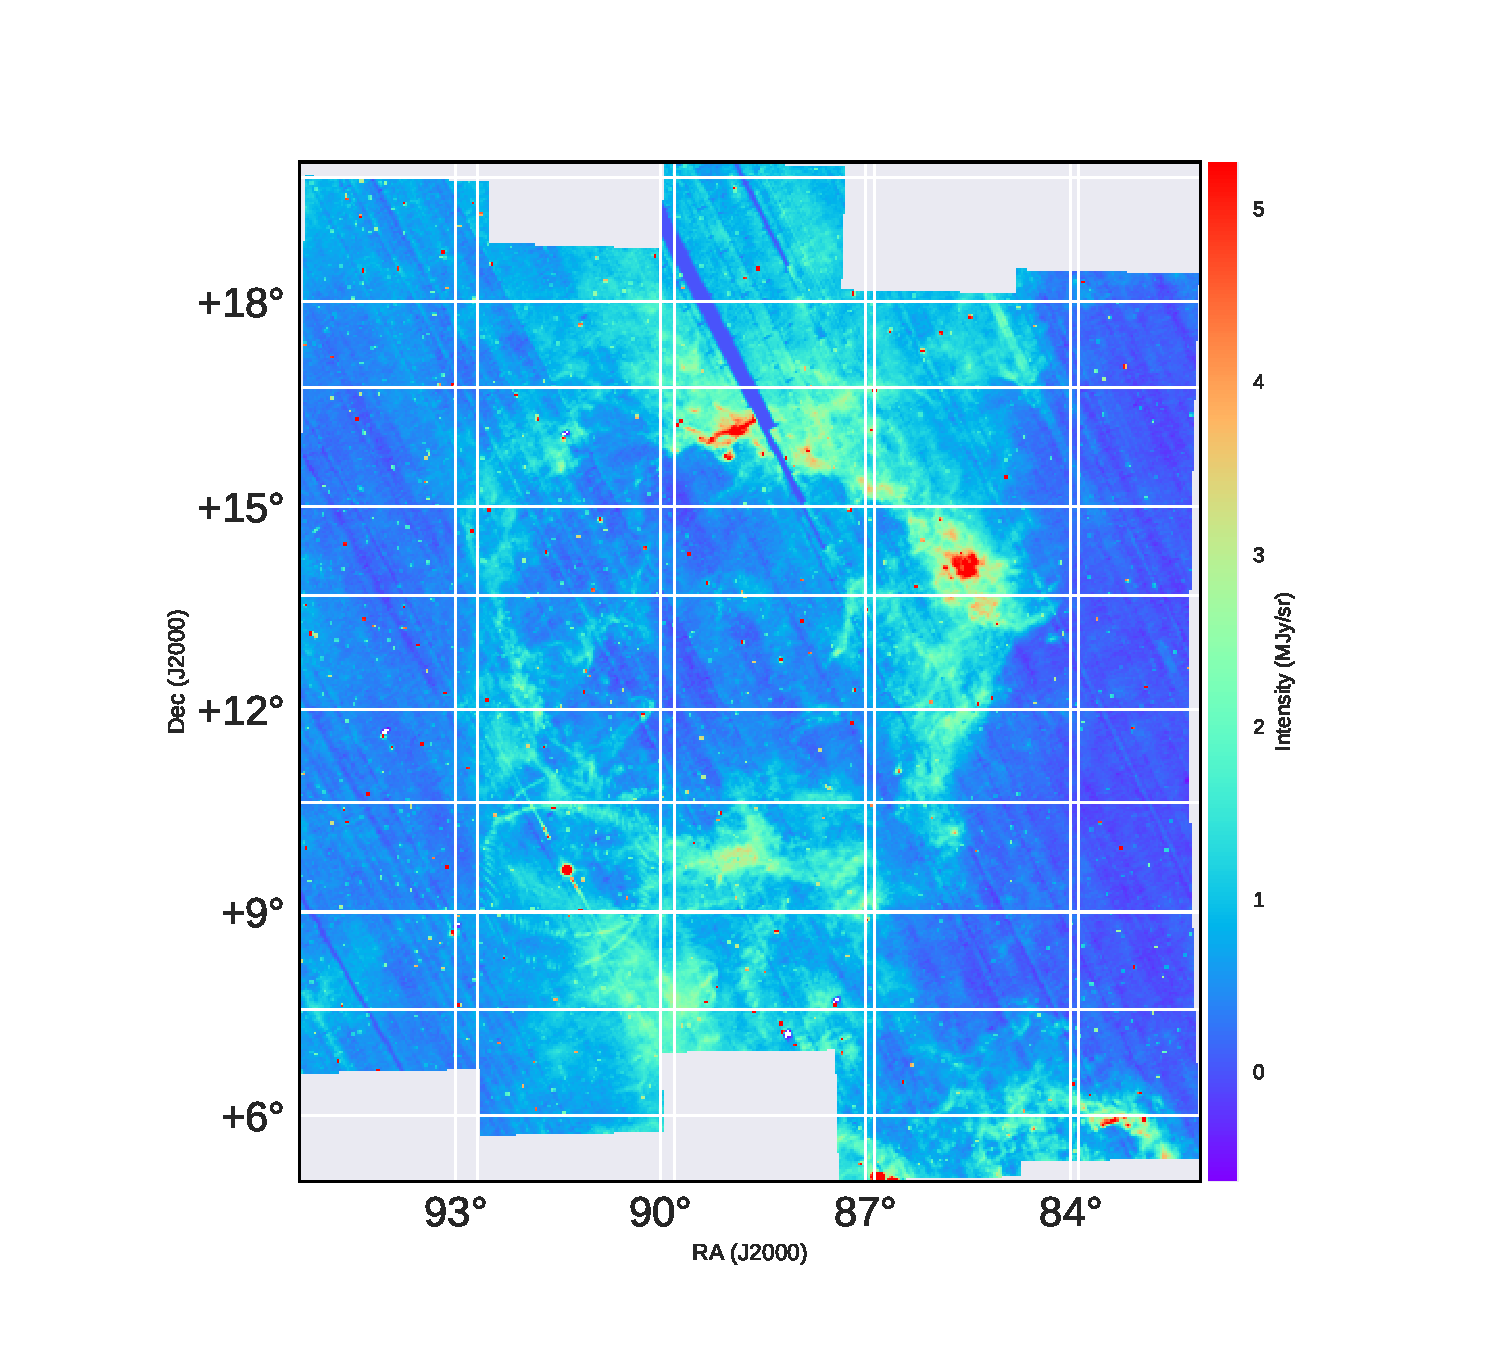
\includegraphics[width=\textwidth,trim={2.5cm 2cm 3.0cm 2cm},clip]{../Plots/ch_lori/lori_A9_mosaic_smooth.pdf}
              \centering
              \caption{The $\lambda$~Orionis region in the A9 band at near-native resolution. This is a mosiac created from the 3x3 degree all-sky survey tiles by Ishirara et al. (in prep.) Missing stripes are less of a problem than with the A18 band (Fig.~\ref{fig:lori_A18_mosaic_smooth}), but point sources are more pronounced. Around Betelgeuse, in the lower left of the image, we can see an artifact caused by scattered light.. }
              \label{fig:lori_A9_mosaic_smooth}
            \end{figure}
            \begin{figure}
              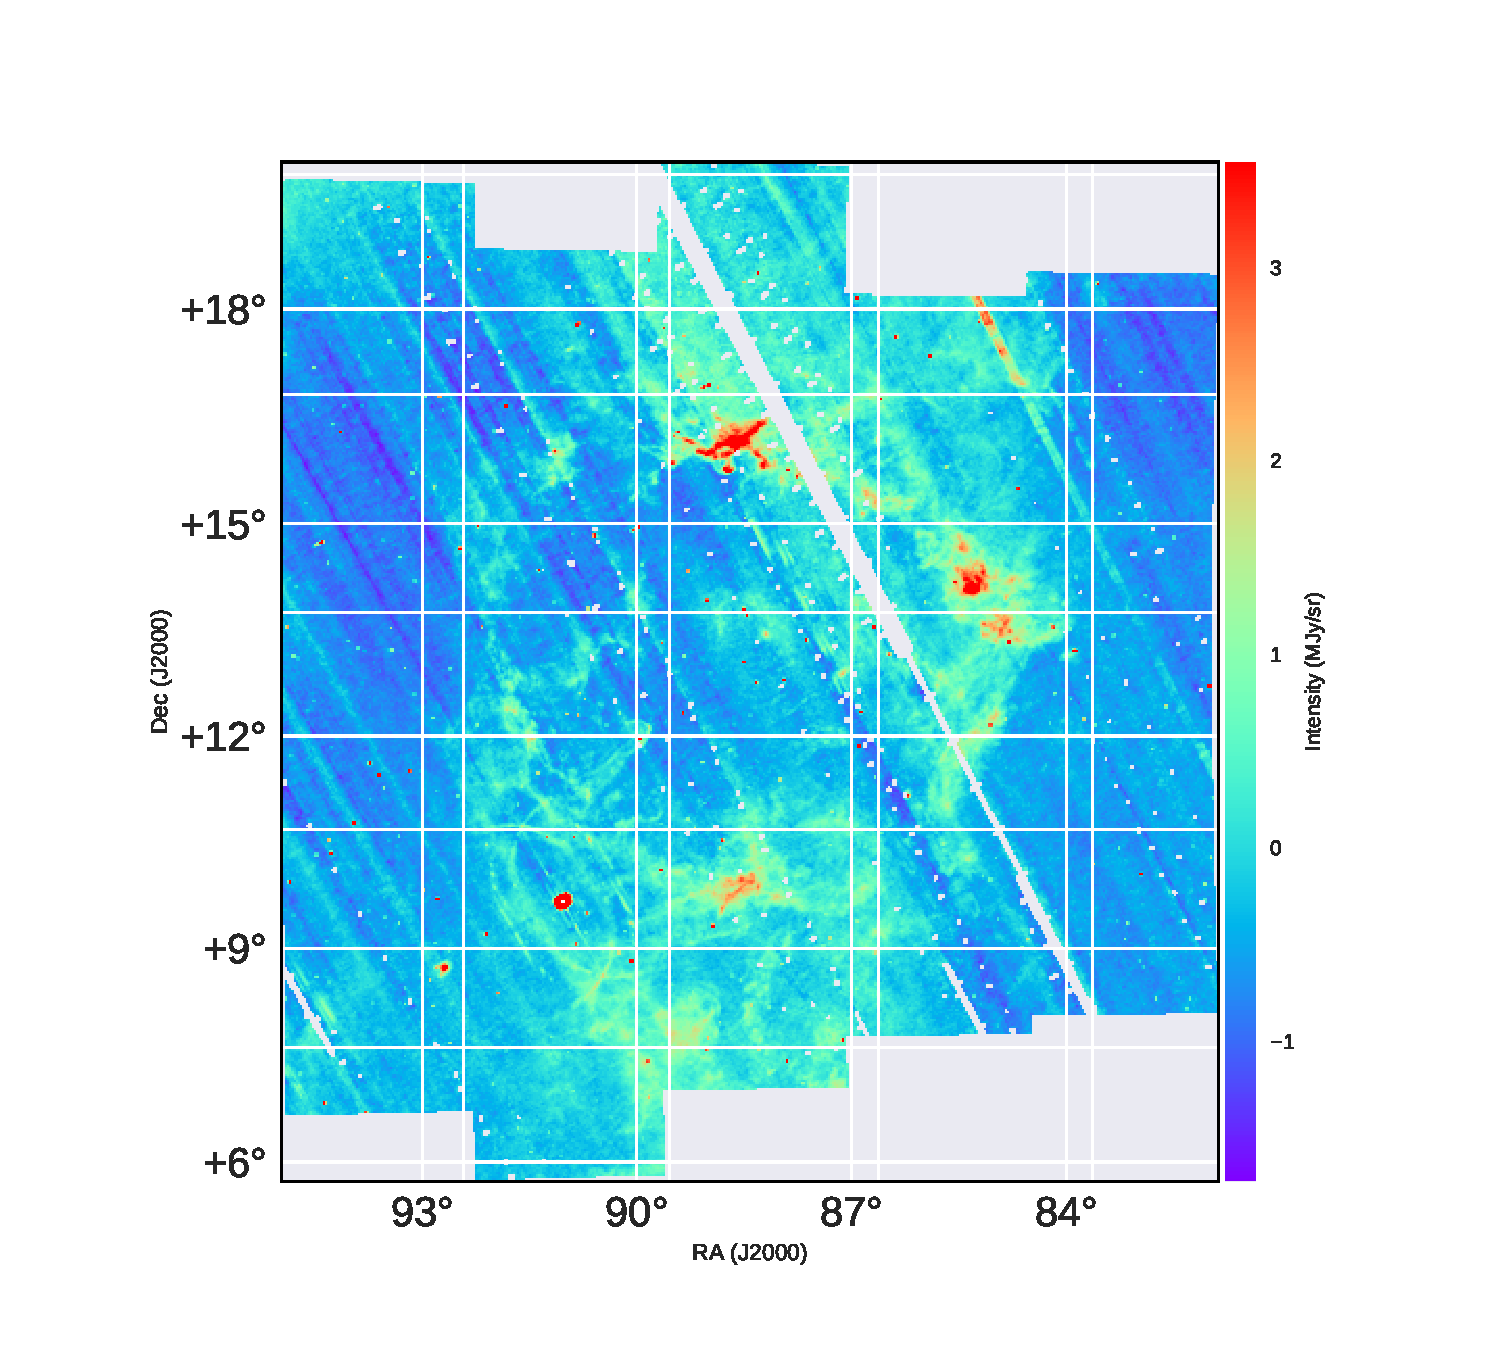
\includegraphics[width=\textwidth,trim={2.5cm 2cm 3.0cm 2cm},clip]{../Plots/ch_lori/lori_A18_mosaic_smooth.pdf}
              \centering
              \caption{The $\lambda$~Orionis region in the A18 band at near-native resolution, demonstrating the regions affected by missing stripe errors, but less affected by point-sources than A9 (Fig.~\ref{fig:lori_A9_mosaic_smooth}). }
              \label{fig:lori_A18_mosaic_smooth}
            \end{figure}

        \paragraph{Point sources}
          A caveat that comes with added ionized \acrshort{pah} feature coverage of the A9 band, is that the shorter central wavelength placement allows more contamination from point sources. We identify point sources with a moving-window approach provided in the astropy Python package, flagging pixels which have higher than 5$\sigma$ intensity among the surrounding 100 pixel window. We then place a mask at the center of the flagged point-sources. The masks are propogated through the regridding step, such that the low-resolution pixels having more than 50\% of their area masked in the high resolution tiles, also become masked. Such pixels appear black in Fig.~\ref{fig:orionis-akari9}. The same process is applied to the A18 data. For other maps, which we extract from HEALPix data, we first regrid from \acrshort{healpix} to rectangular grids, and then apply the point-source search and masking as above. For the I12 and I25 images, the rejected pixels were fewer than with A9, but positions overlapped with those already masked in A9. For bands longer than I25, this process did not result in rejected pixels. For the D12 and D25 bands, which are natively at a much lower resolution than AKARI or \acrshort{dirbe}, point-sources present more of a challenge. For these images, we visually inspect and mask 3 regions with bright point source contamination consistent with the \acrshort{dirbe} beamsize and with point-sources identified in IRAS and IRC images. Pixel positions masked in any single image, are masked in all of the images before the finaly analysis.


        \subsection{PSF Smoothing}
          We smooth the pixels in the spatial domain, to have a 1$^{\circ}$ FWHM PSF, in order to have a resolution approximating that of the \acrshort{pc} \acrshort{ame} data.
          The smoothing process relies on the {\tt convolution} module provided in the {\tt astropy} package. We assume simple circular gaussian kernel for the smoothing process. While they may be asymmetries in the effective beam shapes of the IR bands used, the target resolution of the \acrshort{ame} data is large enough relative to the native resolution of the input IR data (especially A9 and A18, see Fig.~\ref{tab:data}) as to render the beam shapes and positional variations negligible. Finally, we mask pixels along the edge of the FOV where the convolution process produces artifacts.

      \subsection{Background subtraction}
         We estimate an average, flat background level for this region. The background level is determined the mean of pixels in an `OFF` zone. The final images are shown in Fig.~\ref{fig:lori_processed_all}, with the full mask applied (masked pixels are indicated in white), and with the OFF zone indicated by the red rectangle on each frame.
            \begin{figure}
              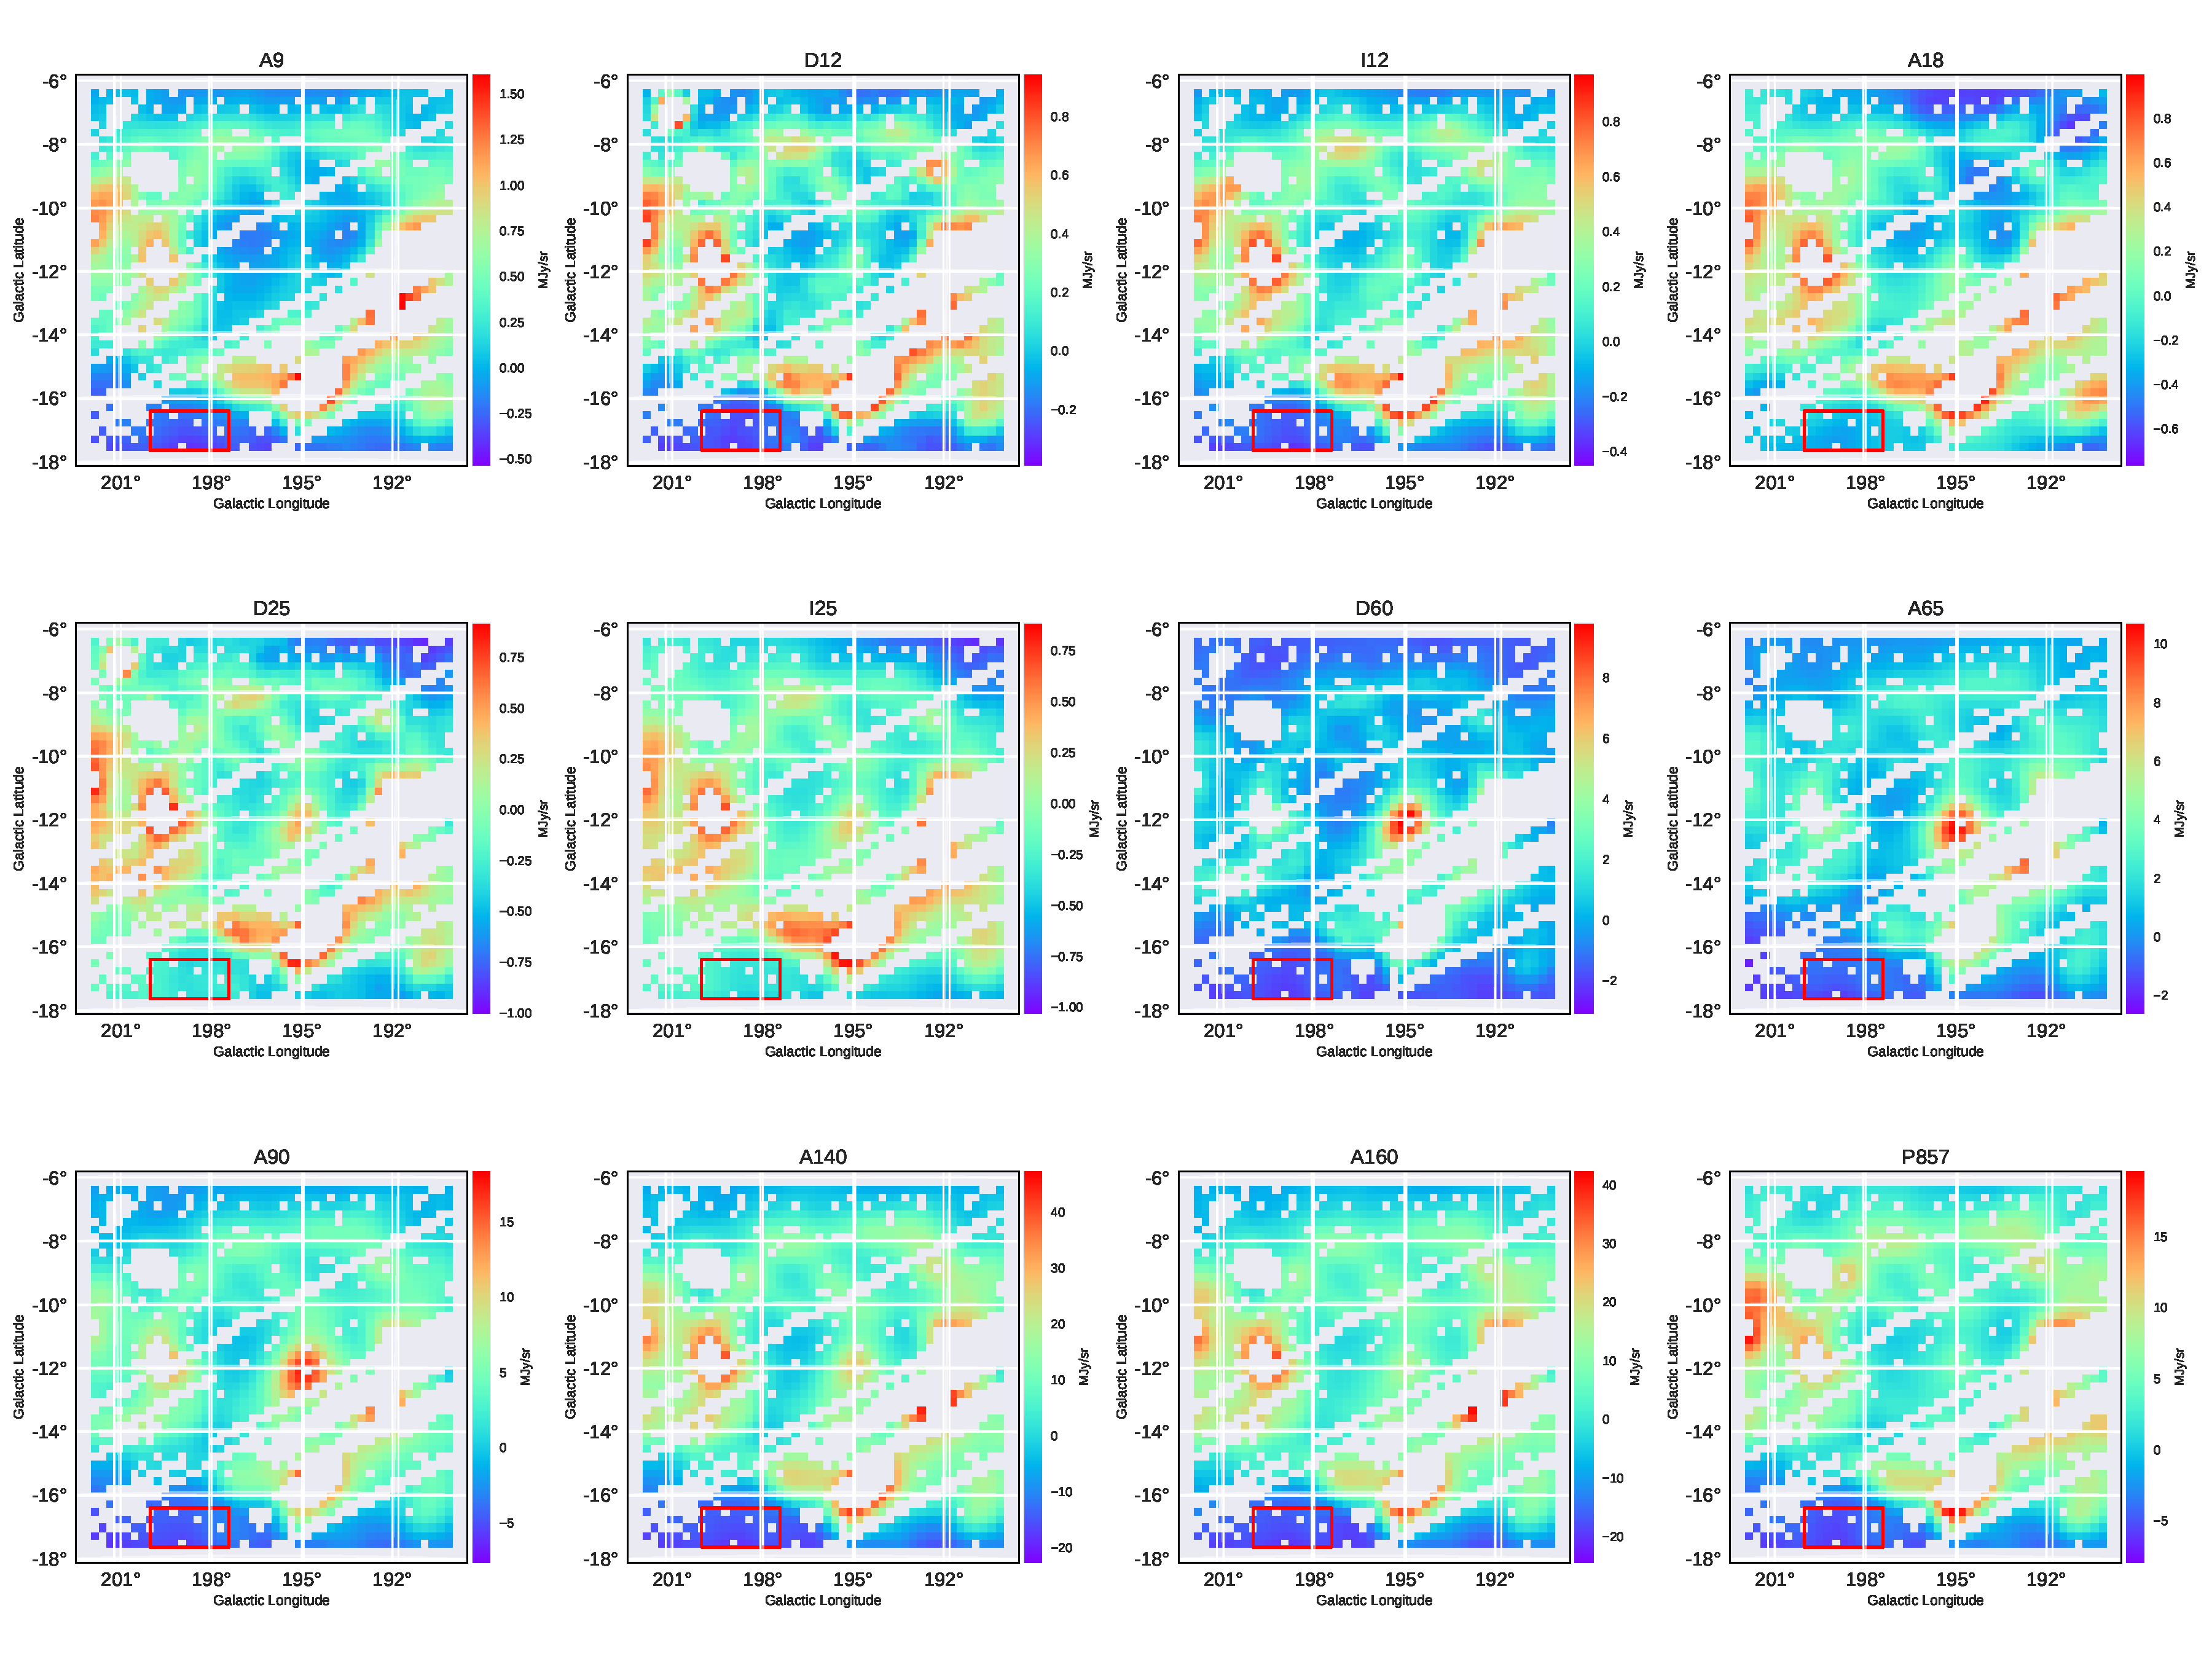
\includegraphics[width=\textwidth,trim={5cm 5cm 3.5cm 5cm},clip]{../Plots/ch_lori/lori_processed_grid.pdf}
              \centering
              \caption{Processed data at each wavelength for $\lambda$~Orionis. A flat background has been subtracted from each frame based on the mean of pixels within the red rectangle. The pixel width is 0.25$^{\circ}$, with the data PSF smoothed to 1$^{\circ}$ spatial resolution. Masked pixels (point sources, stripe errors, convolution artifacts) are shown as white. The frames share the same FOV and GAL-TAN projection. Colorbars indicate the intensity in MJy/sr.}
              \label{fig:lori_processed_all}
            \end{figure}
          We do not expect simple band-by-band intensity correlation tests with the \acrshort{ame} to be sensitive to background and foreground emission along the line of sight towards the $\lambda$~Orionis region. However analyses such as dust \acrshort{sed} fitting, to determine the relative abundances of different dust components, may be effected by the background level. The general morphology as seen in the high resolution AKARI data (Figs.~\ref{fig:LOri_FIS_color},~\ref{fig:lori_A9_mosaic_smooth} and ~\ref{fig:lori_A18_mosaic_smooth}) remains well pronounced in the final, low resolution images.

	\section{Multi-wavelength characterization}
    The correlation matrix results corresponding to data shown in Fig.~\ref{fig:lori_processed_all}, are shown in Fig.~\ref{fig:orionis-corr-matrix}.
      \begin{figure}
        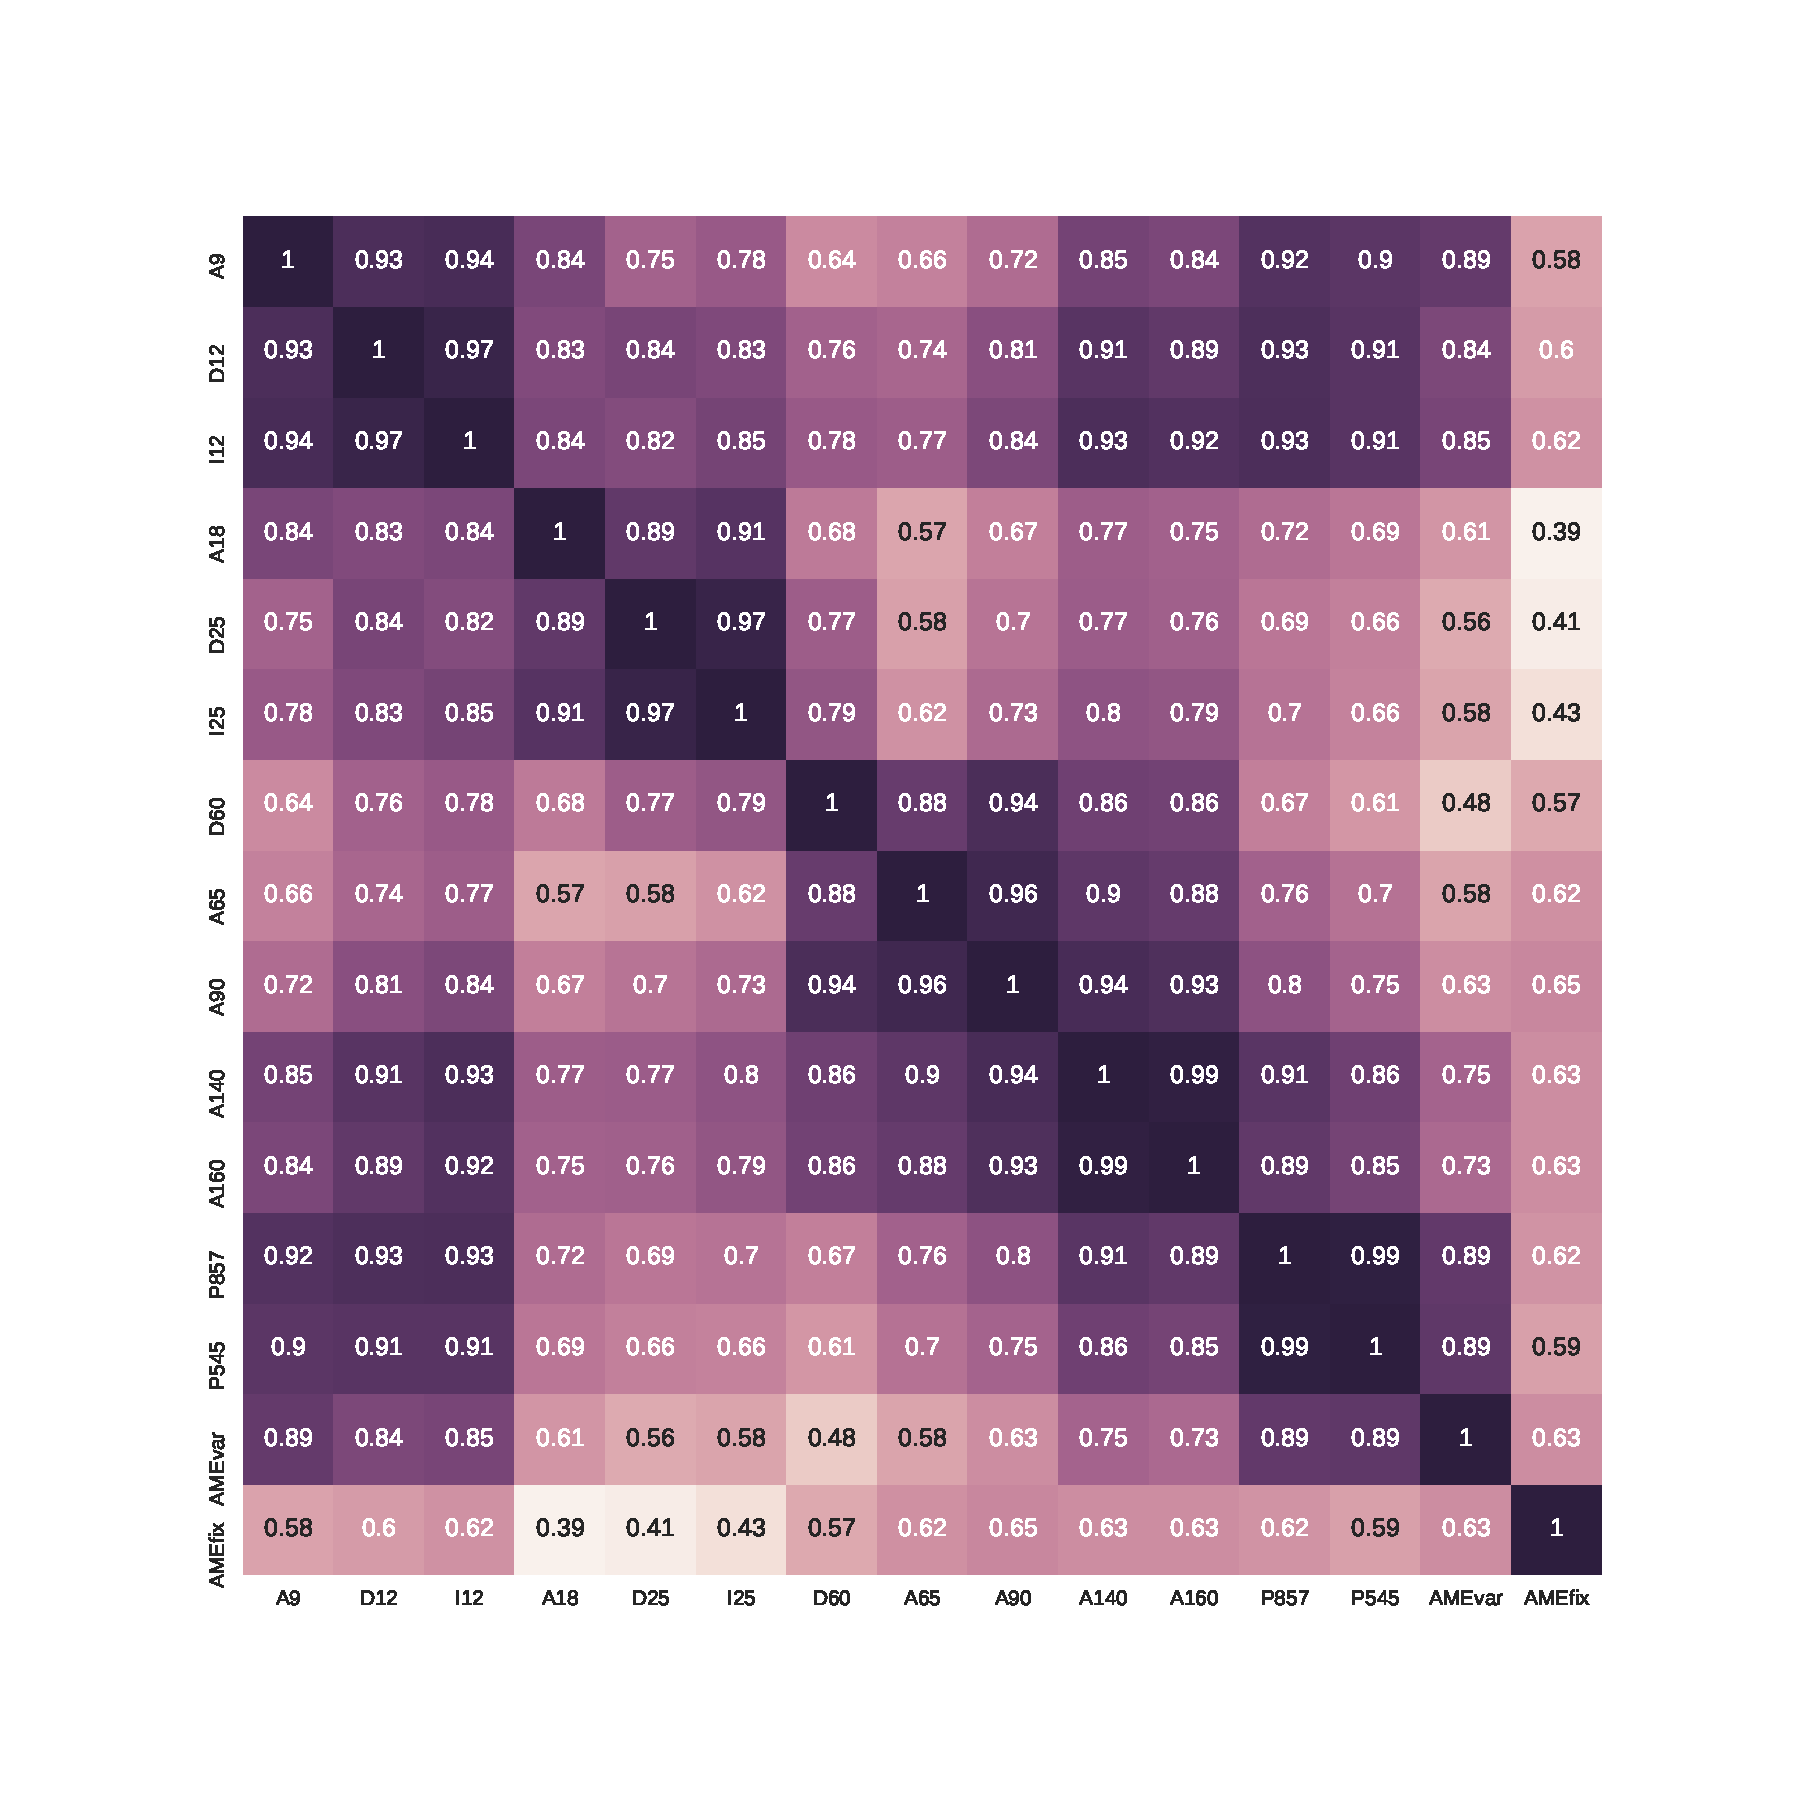
\includegraphics[width=\textwidth]{../Plots/ch_lori/Lori_corrmatrix_I.pdf}
        \centering
        \caption{$r_{s}$ correlation matrix for all of the data used in the $\lambda$~Orionis analysis, similar to that presented for the Planck Commander component maps in Fig.~\ref{fig:PCCS_corrmatrix}. The shade and annotation for each cell indicates the $r_{s}$ score, where $r_{s}$ of 1 indicates a monotonically increasing relationship for a given pair of images. The two \acrshort{ame} components, as described in Ch.~\ref{ch:datasources}, are listed separately: $AME_{var}$ for the frequency-varying component, and $AME_{fix}$ for the constant frequency component.}
        \label{fig:orionis-corr-matrix}
      \end{figure}
     This immediately confirms a correlation between the IR and \acrshort{ame}, however this was readily visibly from the spatial morphology of the region. Interestingly though, the correlation strengths with $AME_{var}$ show a pattern from short to long wavelengths: A9, P857, and P545 show the strongest correlations, with the correlation weaking from A18 to A90, and again strengthening at longer wavelengths. The fixed peak frequency $AME_{fix}$, which is the much fainter component, shows the strongest correlation with A90- though all of the IR correlations relative to $AME_{fix}$ are weaker than those for $AME_{var}$. The overall pattern is for bands dominated by \acrshort{pah} emission (as discussed in Ch.~\ref{ch:datasources}), and those which trace Rayleigh-Jeans thermal dust emission are equally good predictors of the \acrshort{ame}. Bands dominated by a mixture of VSGs, and warm dust emission, show a weaker correlation. For the next stages of analysis, we will consider only the dominant component $AME_{var}$. We found that combining the components does affect the results here.

     Comparing the images in Fig.~\ref{fig:lori_processed_all}, most of the variation in the correlation scores appears to come from the central region of $\lambda$~Orionis. Because of the known heating present within the ring, from the $\lambda$~Orionis association, and given the brightening of bands between A18 and A90, this variation appears to be due to a temperature increase.
    \subsection{Bootstrap analysis}
        To assess the robustness of the correlation scores, we employ the Bootstrap re-sampling approach. We carry out bootstrap correlation tests for each IR band's intensity vs. $AME_{var}$ . The data are resampled 10,000 times for each correlation test, a sufficient resampling given the unmasked pixel count of \textasciitilde{}1400 pixels, and considering that the effective beams are somewhat undersampled.  The distributions of the boostrap resamplings are shown in in Fig.~\ref{fig:bootstrap_vs_AME}.
            \begin{figure}
              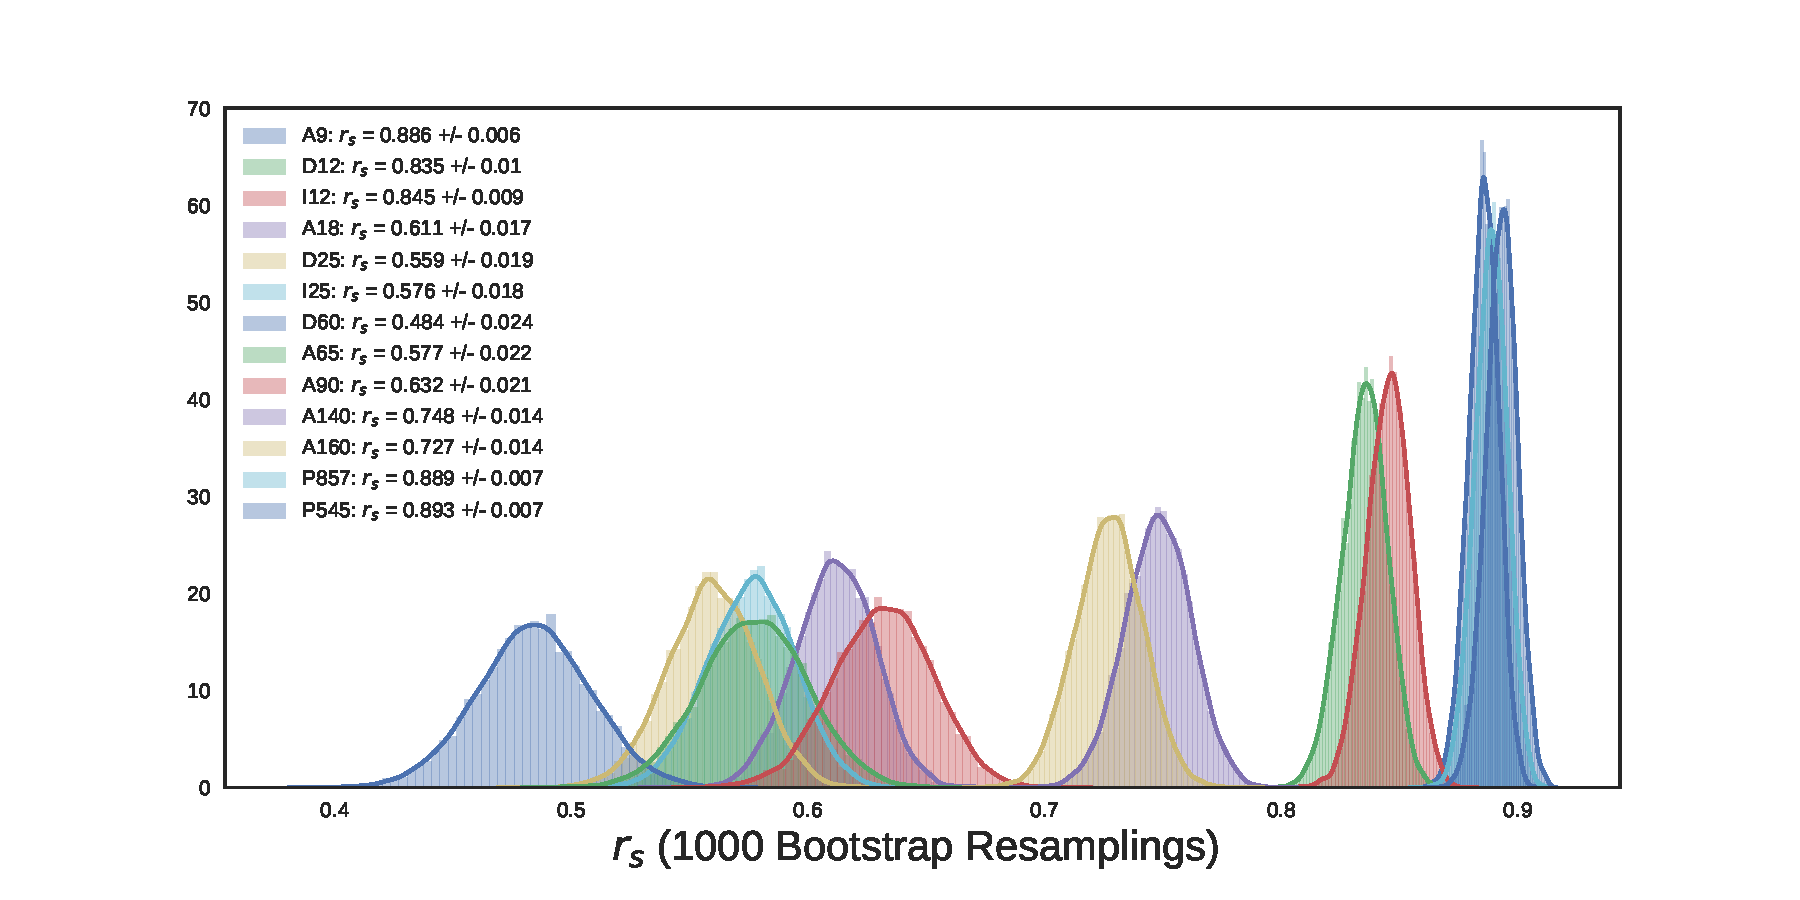
\includegraphics[width=\textwidth,trim={3cm 0.25cm 2.5cm 1cm},clip]{../Plots/ch_lori/bootstrap_vs_AME_spearman_i10000.pdf}
              \centering
              \caption{Re-sampled (Bootstrap) correlation tests for IR emission in $\lambda$~Orionis vs. \acrshort{ame}. Each band's $r_{s}$ distribution is shown in a different color (the same color scheme for both plots). The width of the distribution indicates the error for the given data in the correlation coefficient. The mean and standard deviation of the scores are given in the legend of each plot. The plot ranges only show positive values, since no negative scores were produced. }
              \label{fig:bootstrap_vs_AME}
            \end{figure}
        For both test cases, the best correlations are the longest and shortest wavelength bands, consistent with the straight-forward $r_{s}$ scores shown in Fig.~\ref{fig:orionis-corr-matrix}.

        \section{Comparison with SED Fitting}
          We performed a full dust \acrshort{sed} fitting on the $\lambda$~Orionis photometry, according to the dust model by \cite{galliano11}, and the hierarchical Bayesian SED fitting framework by \cite{galliano18}. There are 4 free paremeters: total dust mass $M_{dust}$, fraction of dust mass as PAHs $q_{PAH}$, the fraction of PAHs that are ionized, and the average strength of the \acrshort{isrf} $U$. As indicated in Ch.~\ref{ch:intro}, we implement such an analysis here primarily because it allows a more careful propgation of the observational errors. We utilize both the \acrlong{hb} approach and a least-squares analysis. The \acrshort{hb} approach allows us to accurately propogate errors in the data (including calibration uncertainties) through the \acrshort{sed} fitting process, as well as the correlation test thereafter. Compared to the ubiquitous \acrlong{lsm} In traditional \acrshort{sed} fitting we often assume only Gaussian uncorrelated noise. Even if this were a valid assumption for the raw data, processing steps may induce correlations or skew noise. Induced correlations may also appear in the parameters fit via standard approaches, when environments are mixed along the line-of-sight \citep{shetty09}.

         We used a mixture of silicate and carbonaceous dust, silicate dust, the two dominant categories of interstellar dust as described in Ch.~\ref{ch:intro}. However, instead of the graphite-based carbon dust invoked by the canonical \cite{draine07} model (DL07), we assume amorphous carbon. This is an attempt to account for an excessive dust-gas-ratio, reported by \cite{israel10, bot10} in the \acrlong{lmc}, which was found by \cite{galliano11} to violate elemental depletion constraints. The increased opacity of amorphous carbon (a factor of 2-3 more than DL07) allows a better fit to \acrshort{herschel} observations of the \acrshort{lmc} \citep{galliano11}, and Planck observations of the Milky Way \citep{planckIntXXIX16}. We assume that the radiation field heating this dust mixture takes the profile of the typical Galactic \acrshort{isrf} in \cite{mathis83}.

          We only carry out the fitting for unmasked pixels. We are primarily interested in which of the corrleations $M_{dust}$ vs. $I_{AME}$ or $M_{PAH}$ vs. $I_{AME}$ is stronger.

          Two sample \acrshort{sed} fitting results are shown in Figs.~\ref{fig:fred_LOri_notes_Oct2017_fig1a}, and~\ref{fig:fred_LOri_notes_Oct2017_fig1b}.
              \begin{figure}
                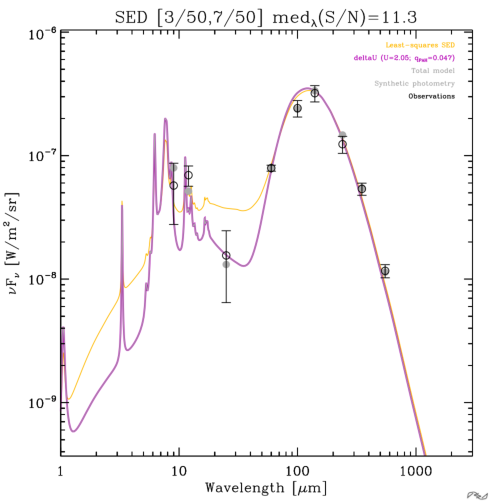
\includegraphics[width=\textwidth]{../Plots/ch_lori/fred_LOri_notes_Oct2017_fig1a.pdf}
                \centering
                \caption{Observed (black circles and errors) and synthetic photometry (gray dots) \acrshort{sed} of a pixel within $\lambda$~Orionis, along with the dust \acrshort{sed} model fit results. Two \acrshort{sed} fits are shown: on for the Bayesian fitting (magenta), and another showing the standard least-squares result for comparison (yellow). The fitted \acrshort{isrf} strength $U$, and fraction of mass in \acrshort{pah}s, $q_{PAH}$ are also given.}
                \label{fig:fred_LOri_notes_Oct2017_fig1a}
              \end{figure}
              \begin{figure}
                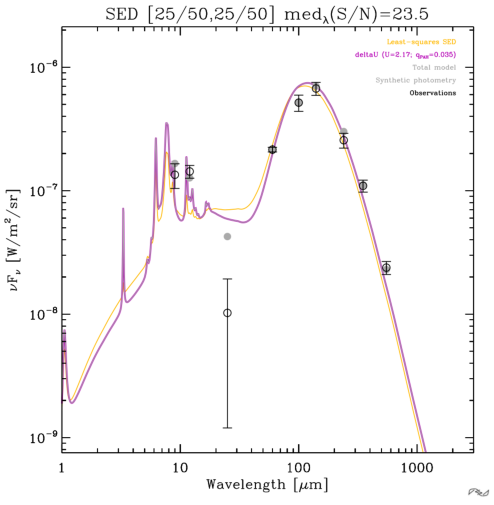
\includegraphics[width=\textwidth]{../Plots/ch_lori/fred_LOri_notes_Oct2017_fig1b.pdf}
                \centering
                \caption{The same as Fig.~\ref{fig:fred_LOri_notes_Oct2017_fig1a}, but for a different pixel position.}
                \label{fig:fred_LOri_notes_Oct2017_fig1b}
              \end{figure}
           Performing such fits for all of the pixels, we are able to see how $I_{AME}$ varies with the dust properties of the region. Fig.~\ref{fig:corr_IameUav_lnMd} shows the fitted dust mass per pixel, relative to the \acrshort{ame} intensity.
                \begin{figure}
                 \includegraphics[width=\textwidth]{../Plots/ch_lori/corr_IameUav_lnMd.pdf}
                 \centering
                 \caption{Scatter plot with the bivariate error elipses generated through the \acrshort{hb} \acrshort{sed} fitting, of total dust mass $M_{dust}$ vs. $I_{AME}$ scaled by $U$. Green dots indicate the results when using a simple least-squares method fit, for comparison with the HB method.}
                 \label{fig:corr_IameUav_lnMd}
               \end{figure}
           \acrshort{ame} intensity is scaled by the \acrshort{isrf} intensity $U$. Although spinning dust emission is not predicted to vary directly with $U$, we consider that the ISRF may serve as a diagnostic of environmental conditions in the \acrshort{ism}. In any case, we find that performing such a scaling improves the correlations with dust mass.   Figs.~\ref{fig:corr_IameUav_lnMpah} and~\ref{fig:corr_IameUav_lnMpahion} describe the variation with $M_{PAH}$ and $M_{PAH+}$.
              \begin{figure}
                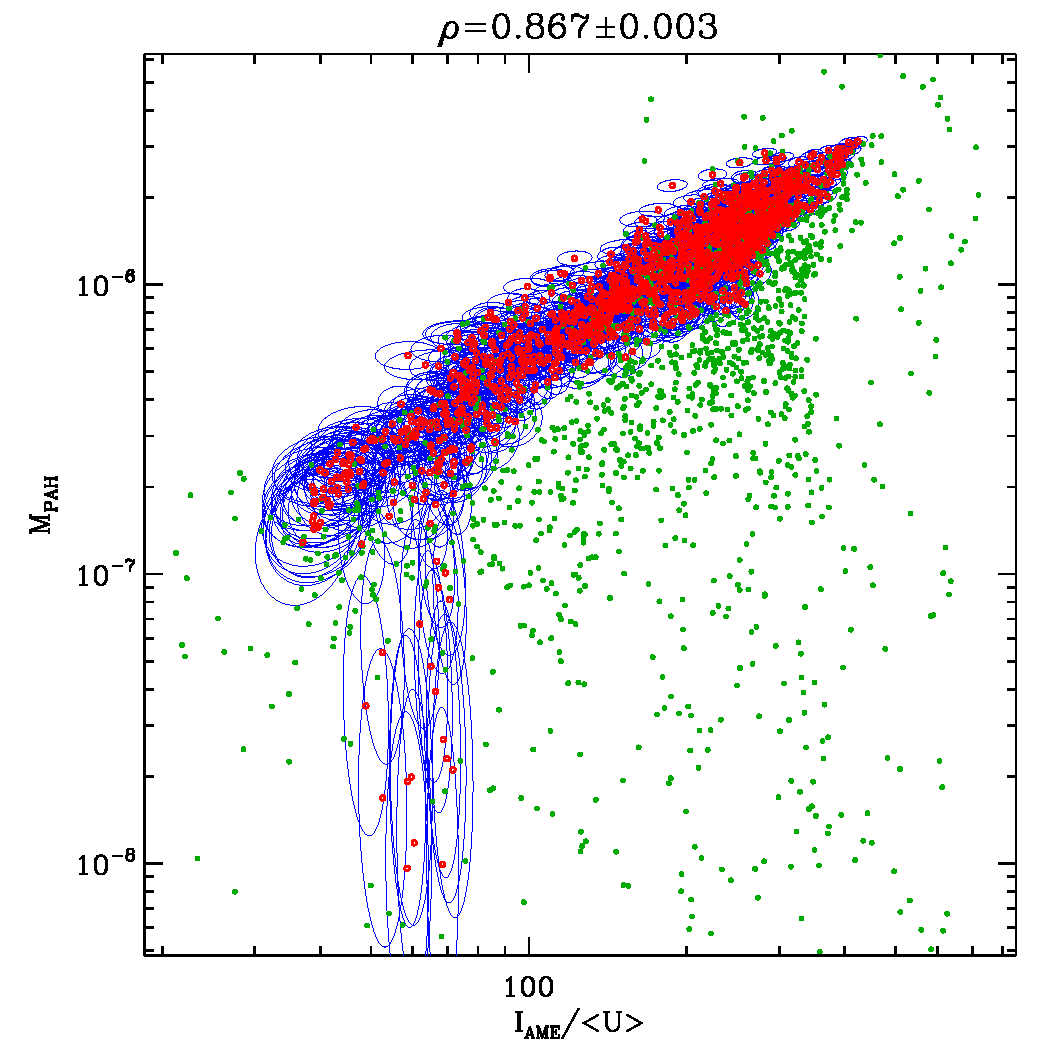
\includegraphics[width=\textwidth]{../Plots/ch_lori/corr_IameUav_lnMpah.pdf}
                \centering
                \caption{The same comparison is given by~\ref{fig:corr_IameUav_lnMd}, but showing total mass of \acrshort{pah}s ($M_{PAH}$) rather than total dust mass on the y-axis. }
                \label{fig:corr_IameUav_lnMpah}
              \end{figure}
              \begin{figure}
                \includegraphics[width=\textwidth]{../Plots/ch_lori/corr_IameUav_lnMpahion.pdf}
                \centering
                \caption{ The same as in Figs.~\ref{fig:corr_IameUav_lnMd} and~\ref{fig:corr_IameUav_lnMpah}, but specifically comparing an estimate of the charged component of \acrshort{pah} mass $M_{PAH+}$. This includes anions and cations, since we cannot distinguish between these two spectroscopically.}
                \label{fig:corr_IameUav_lnMpahion}
              \end{figure}
    Based on the dust properties derived from these \acrshort{sed} fits, we investigate whether any fitted parameter shows a preferential relation with the \acrshort{ame}. Figs.~\ref{fig:corr_IameUav_lnMd}-\ref{fig:corr_IameUav_lnMpahion} reveal a very similar trend between the \acrshort{ame} and the parameters $M_{PAH}$, $M_{PAH+}$, and $M_{dust}$. There is a slightly improved correlation between $M_{dust}$ and $M_{PAH}$ (0.857 vs 0.867). This is consistent with the intensity cross correlations in Fig.~\ref{fig:orionis-corr-matrix}. These corrleations are discussed further in Sec.~\ref{sec:lori_discussion} and Fig.~\ref{fig:PDFs_Iame}.

    \subsection{Comparing the Correlation Strengths}

    In addition to probability distribution functions of the fitted parameters, HB allows us to plot the final PDFs of the correlation coefficients themselves. This is a more robust way of comparing the correlation strengths than simply bootstrapping the correlations. Fig.~\ref{fig:PDFs_Iame} shows the $r_{s}$  PDFs for the 3 major correlations of interest: $r_{s}(I_{AME},M_{dust})$, $r_{s}(I_{AME},M_{PAH})$, and $r_{s}(I_{AME},M_{PAH+})$.
        \begin{figure}
          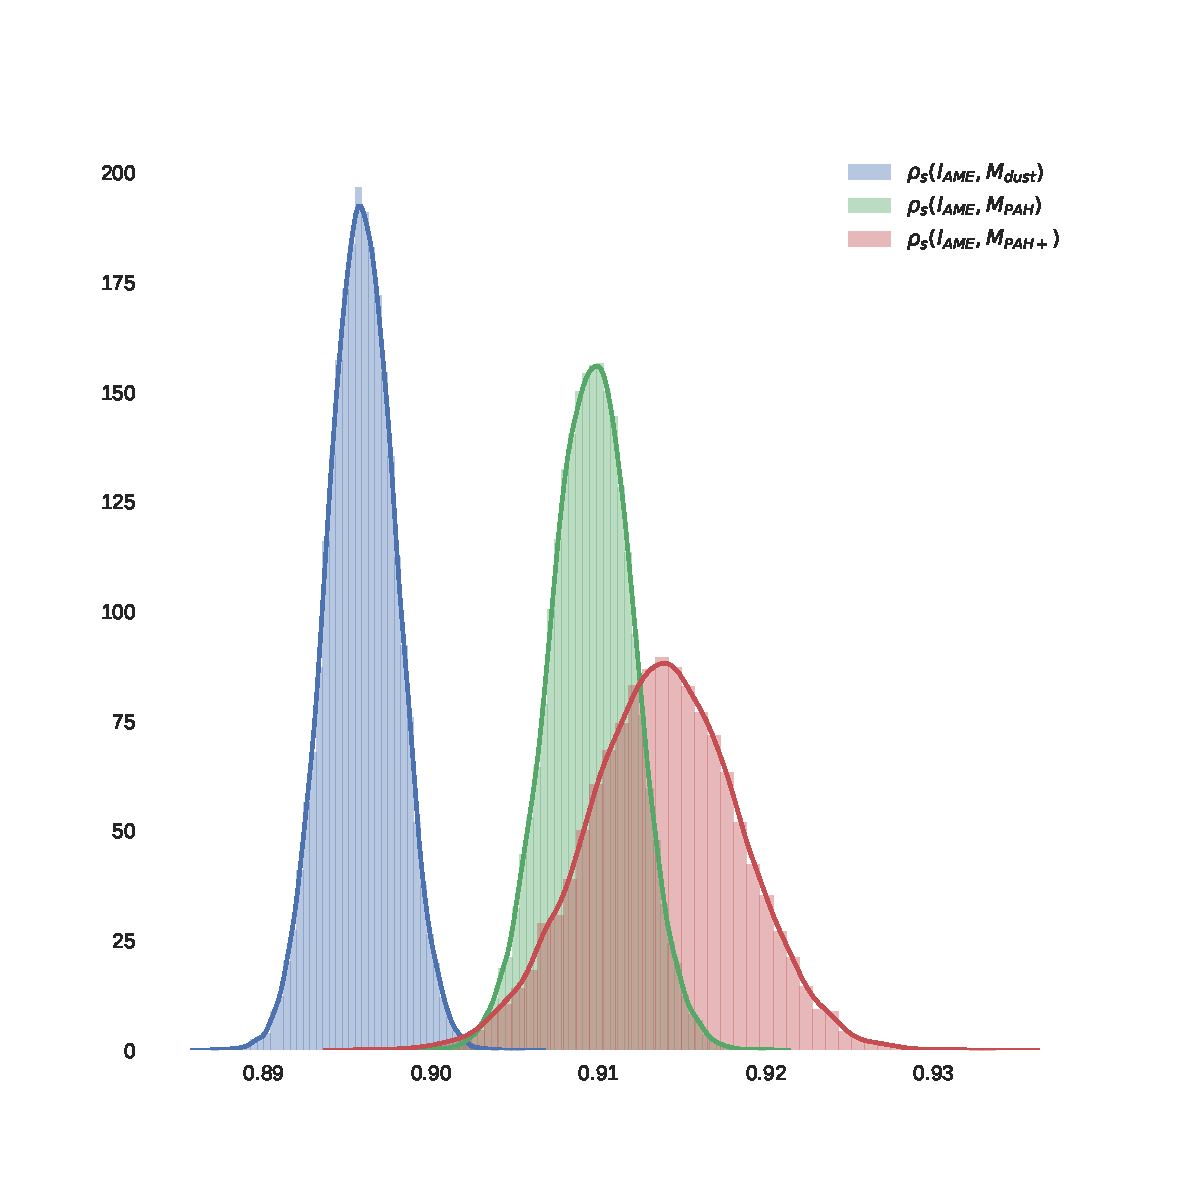
\includegraphics[width=\textwidth]{../Plots/ch_lori/PDFs_Iame.pdf}
          \centering
          \caption{ The hierarchical Bayesian correlation probablity distributions of $r_{s}$) for the three physical parameters vs. the \acrshort{ame} intensity: total dust mass, $r_{s}(dust)$ (blue); total \acrshort{pah} mass $r_{s}(PAH)$ (green); and only the ionized \acrshort{pah} mass $r_{s}(PAH+)$ (red). Also given are the probabilities of either \acrshort{pah} component being better correlated with \acrshort{ame} than dust mass, as well as the probability that ionized \acrshort{pah} mass correlates better than total \acrshort{pah}.}
          \label{fig:PDFs_Iame}
        \end{figure}
    To assess the effect of the morphology of $\lambda$~Orionis on these results, we show the same PDFs but omitting the central region of $\lambda$~Orionis. This is shown in Fig.~\ref{fig:PDFs_center_masked_Iame}.
         \begin{figure}
          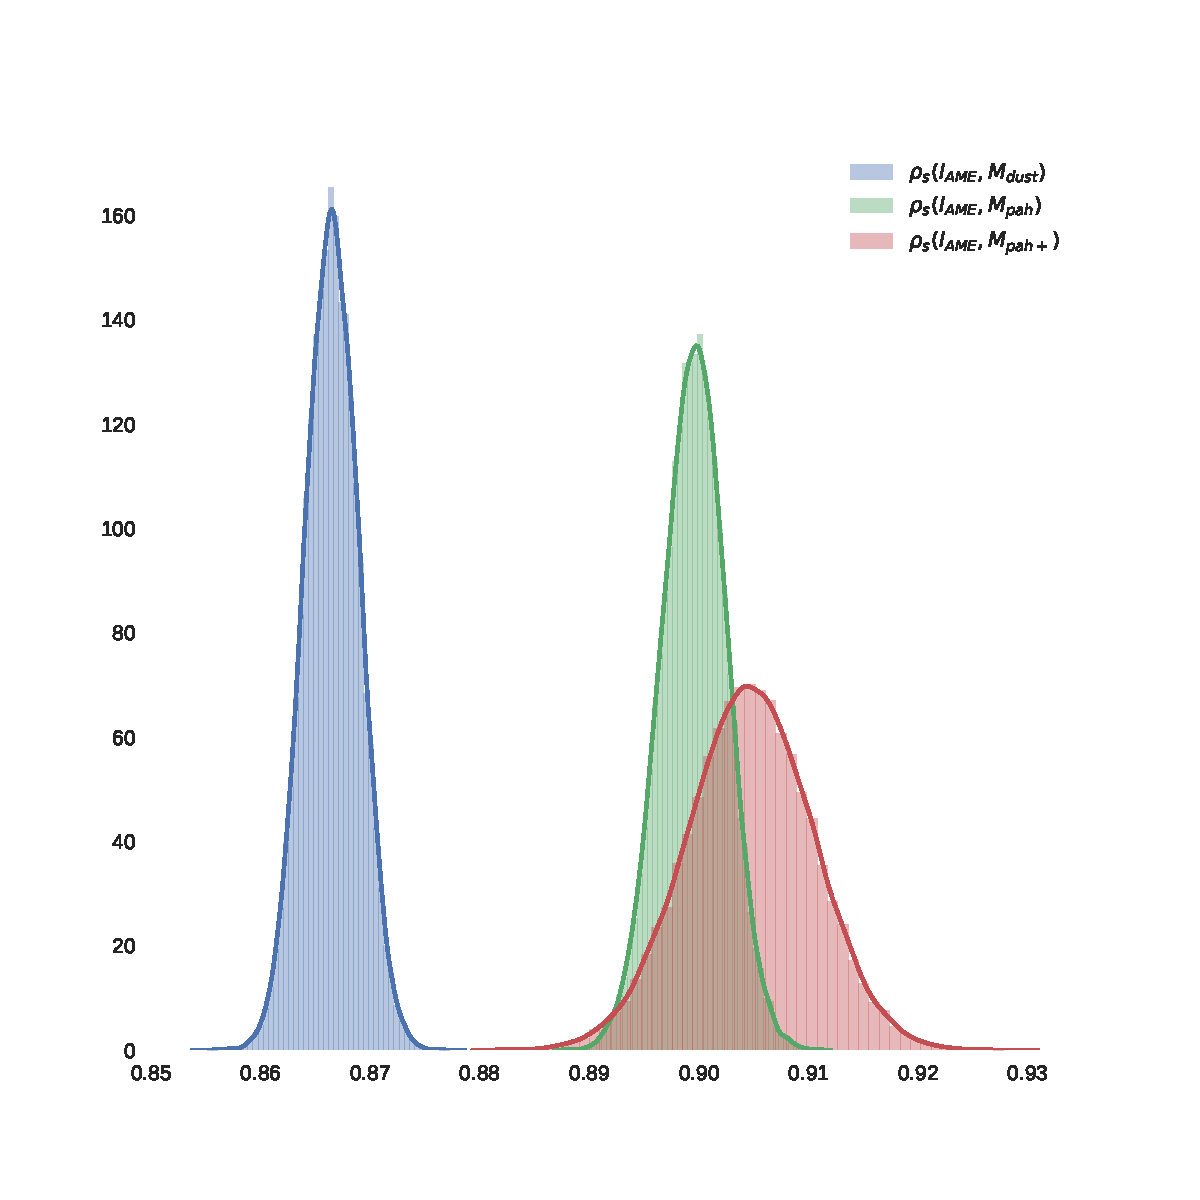
\includegraphics[width=\textwidth]{../Plots/ch_lori/PDFs_center_masked_Iame.pdf}
          \centering
          \caption{ The hierarchical Bayesian correlation coefficent ($r_{s}$ as shown in PDFs as shown in Fig.~\ref{fig:PDFs_Iame}, but with the central region of $\lambda$~Orionis masked, according to Fig.~\ref{fig:lambda_orionis_center_mask}. }
          \label{fig:PDFs_center_masked_Iame}
        \end{figure}
    The extent of the mask is indicated in Fig~\ref{fig:lambda_orionis_center_mask}.
        \begin{figure}
          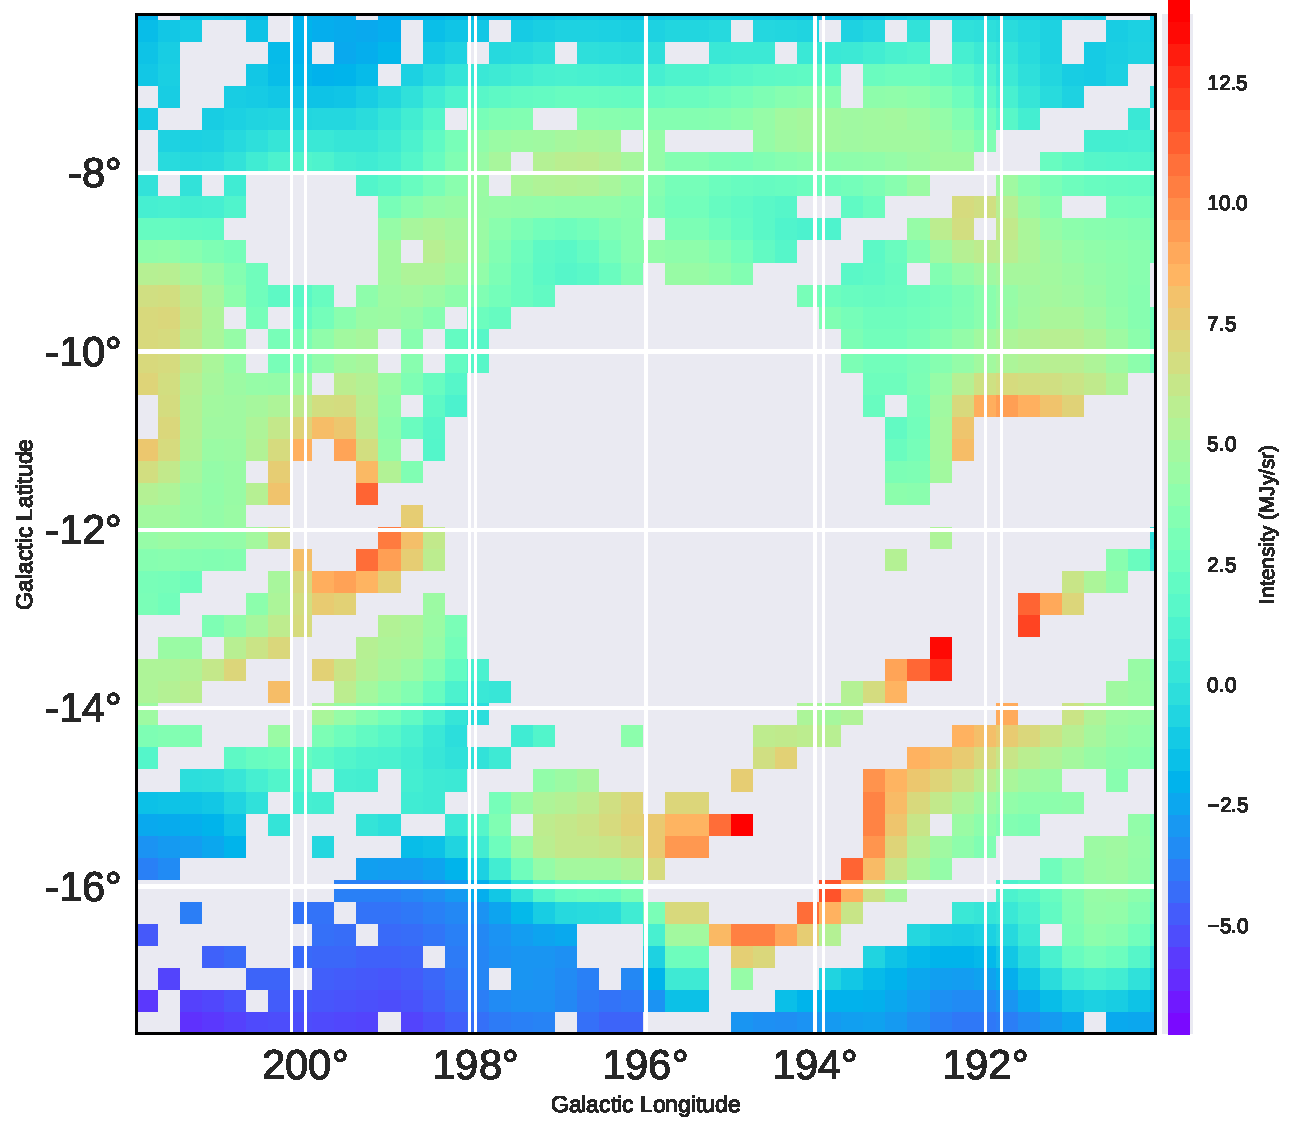
\includegraphics[width=\textwidth]{../Plots/ch_lori/lambda_orionis_center_mask.pdf}
          \centering
          \caption{ The A90 image of $\lambda$~Orionis shown to demonstrate the mask applied to the central region, in order to produce the PDFs in Fig.~\ref{fig:PDFs_center_masked_Iame}. The region showing an apparent dust temperature peak, which was most prominent in the A90 image and the major point of variation accross all the wavelengths, is thus omitted.}
          \label{fig:lambda_orionis_center_mask}
        \end{figure}

  \section{Discussion}
  \label{sec:lori_discussion}
      In  $\lambda$~Orionis we found that accross the whole region, A9 emission and P545 emission were the most strongly correlated with \acrshort{ame}. This is apparent both in the photometric band analysis, and in the dust \acrshort{sed} fitting.  The fact that the correlation strengths of \acrshort{pah}-tracing mission and sub-mm emission are similar is in-line with what we have seen in \cite{ysard10b} and \cite{hensley16}. In those works, the two relationships (\acrshort{mir} vs. \acrshort{ame} and \acrshort{fir} vs. \acrshort{ame}) are very close, although these two papers are odds as to which relationship is stronger, and thus in their final interpretation. With the present data and analysis of $\lambda$~Orionis, we fail to rule out \acrshort{pah}s as carriers of the \acrshort{ame}. In fact, our primary result, shown in Fig.~\ref{fig:PDFs_Iame} indicates that PAH mass is a stronger predictor of the AME, compared to the total dust mass. This is the first time such a significant result has been found, in support of the PAH hypothesis for a particular region. This core result is unchanged even when we examine the outer ring structure separately from the central region, as shown in Fig.~\ref{fig:PDFs_center_mask_Iame}.

        The results are consistent with a scenario in which \acrshort{pah} mass, cold dust, and the \acrshort{ame} are tightly correlated. A correlation between cold dust and \acrshort{pah}s is observed in extragalactic targets \citep{haas02}, and may be inferred from the correlation between \acrshort{uir} and \acrshort{fir} emission reported in diffuse galactic \acrshort{ism} \citep{onaka96}. In the case that \acrshort{ame} emanenates from spinning \acrshort{pah}s, it is not surprising that cold dust would also correlate with the \acrshort{ame}. Weaker correlation from 25 to 70~$\mu$m may indicate that \acrshort{ame} is weaker in regions of warmer dust and stronger radiation fields. Such an anti-correlation with harsher radiation are consistent with the carriers of \acrshort{ame} being destroyed in the central region of $\lambda$~Orionis, thus leading to substantially decreased spinning dust emission.

      \subsection{Performance of the Hierarchical Bayesian Fitting}


      Indicated in Figs.~\ref{fig:corr_IameUav_lnMd}, \ref{fig:corr_IameUav_lnMpah}, and\ref{fig:corr_IameUav_lnMpahion}, the trends described in this chapter between dust mass and \acrshort{pah} mass, and the \acrshort{ame} intensity were revealed through the \acrshort{hb} analysis. The increased scatter of best-fit points, produced by the least-squares analysis, obviously obscures the intrinsic relationships. With only \acrshort{lsm} results, the dust \acrshort{sed} fitting comparison would have been inconclusive. To our knowledge, this is the first case of the \acrshort{hb} approach being applied to a localized investigation of \acrshort{ame}, and certainly the first time that the dust \acrshort{sed} of $\lambda$~Orionis region has been investigated in such a way. This raises questions about the future of \acrshort{lsm}-based analysis in dust \acrshort{sed} studies, and highlights the potential this \acrshort{hb} framework developed by \cite{galliano18}.


      \subsection{PAH Ionization fraction}
          As described in Ch.\ref{ch:datasources} it is expected that relative variations between the A9 and I12 intensities could be explained by the fraction of \acrshort{pah}s that are charged, $fPAH+$. Spectroscopically, we cannot distinguish between \acrshort{pah} anions or cations. However if spinning dust emission arises from anions, a better correlation with the mass of charged \acrshort{pah}s $M_{PAH+}$ is expected. However if the \acrshort{pah}s are positively charged, a stronger correlation with $M_{PAH+}$ is not expected. This is due to the rotational excitability of the \acrshort{pah}s: anions are more succeptable to rotational excitation by $H^{+}$ and $C^{+}$ collisions\citep{ali-haimoud10}.

          Examining $\lambda$~Orionis in intensity, we find that the A9 intensity correlates more strongly with \acrshort{ame} than I12 or D12. In the $r_{p}$ case, A9 correlates more strongly with \acrshort{ame} than any other band. This is consistent with the spinning \acrshort{pah} hypothesis, and taken alone may indicate that the 6.2~$\mu$m feature emission from charged \acrshort{pah}s, may be a better predictor of \acrshort{ame} intensity.

          As shown by the dust \acrshort{sed} fitting however, the probability distributions (Fig.~\ref{fig:PDFs_Iame}) of $r_{p}(M_{PAH+}:I_{AME})$ do not indicate that ionized \acrshort{pah} mass correlates better with the total \acrshort{pah} mass. Attempts to estimate the $M_{PAH+}$ based on the available data appear to only add noise relative to $r_{p}(M_{PAH}:I_{AME})$. The means of the two distrubtions $r_{p}(M_{PAH+}:I_{AME})$  and $r_{p}(M_{PAH}:I_{AME})$ are similar and $r_{p}(M_{PAH+}:I_{AME})$ shows a wider distribution. Thus the question of whether or not \acrshort{ame} comes predominantly from charged \acrshort{pah}s remains open.

          The fact that A9 correlates more strongly than the 12~$\mu$m bands, at least suggests that this topic is worth further investigation. What is clear from the \acrshort{mir} and \acrshort{ame} morphology however, is that there is a transition from a relatively \acrshort{pah} depleted, warmer, stronger \acrshort{isrf} in the centerand warm dust in the center to a \acrshort{pah}-supporting region in the ring. Along this transition, there must be a decreasing radiation field with distance from dimnant heating sources, in $\lambda$~Orionis association. \cite{andrews16} predict a transition of \acrshort{pah} species along such a radiation field gradient, from complete \acrshort{pah} destruction in harsh environments, to survival of (sufficiently large) \acrshort{pah} anions near the surface of molecular clouds. Thus if our stronger correlation with A9 indicates charged \acrshort{pah}s, this could be consistent with \acrshort{pah} anions surviving in the portions of $\lambda$~Orionis which are emitting the strongest \acrshort{ame}. Future wide-area spectral mapping of the ${\lambda}$~Orionis region may be able to conclusively test for increased $fPAH+$ in regions with stronger \acrshort{ame}. This would also help us to understand the extent to which [NeII] emission may contribute to the I12 emission, and if this may lead to a relatively improved correlation between \acrshort{ame} and A9. Such studies would be strongly aided by higher resolution probing of spatial variations the \acrshort{ame} spectral profile.
